\documentclass[11pt]{article}
%Gummi|065|=)
\usepackage[utf8]{inputenc}
\usepackage{graphicx}
\title{\textbf{Annexe}}
\author{Max Halford\\
		Giovanni Zanitti\\}
\date{}
\begin{document}

\maketitle

\pagebreak

\section{Genre(s) des films | Catégorie d'âge des utilisateurs}
\subsection{Femmes}
\begin{figure}[htd]
\centering
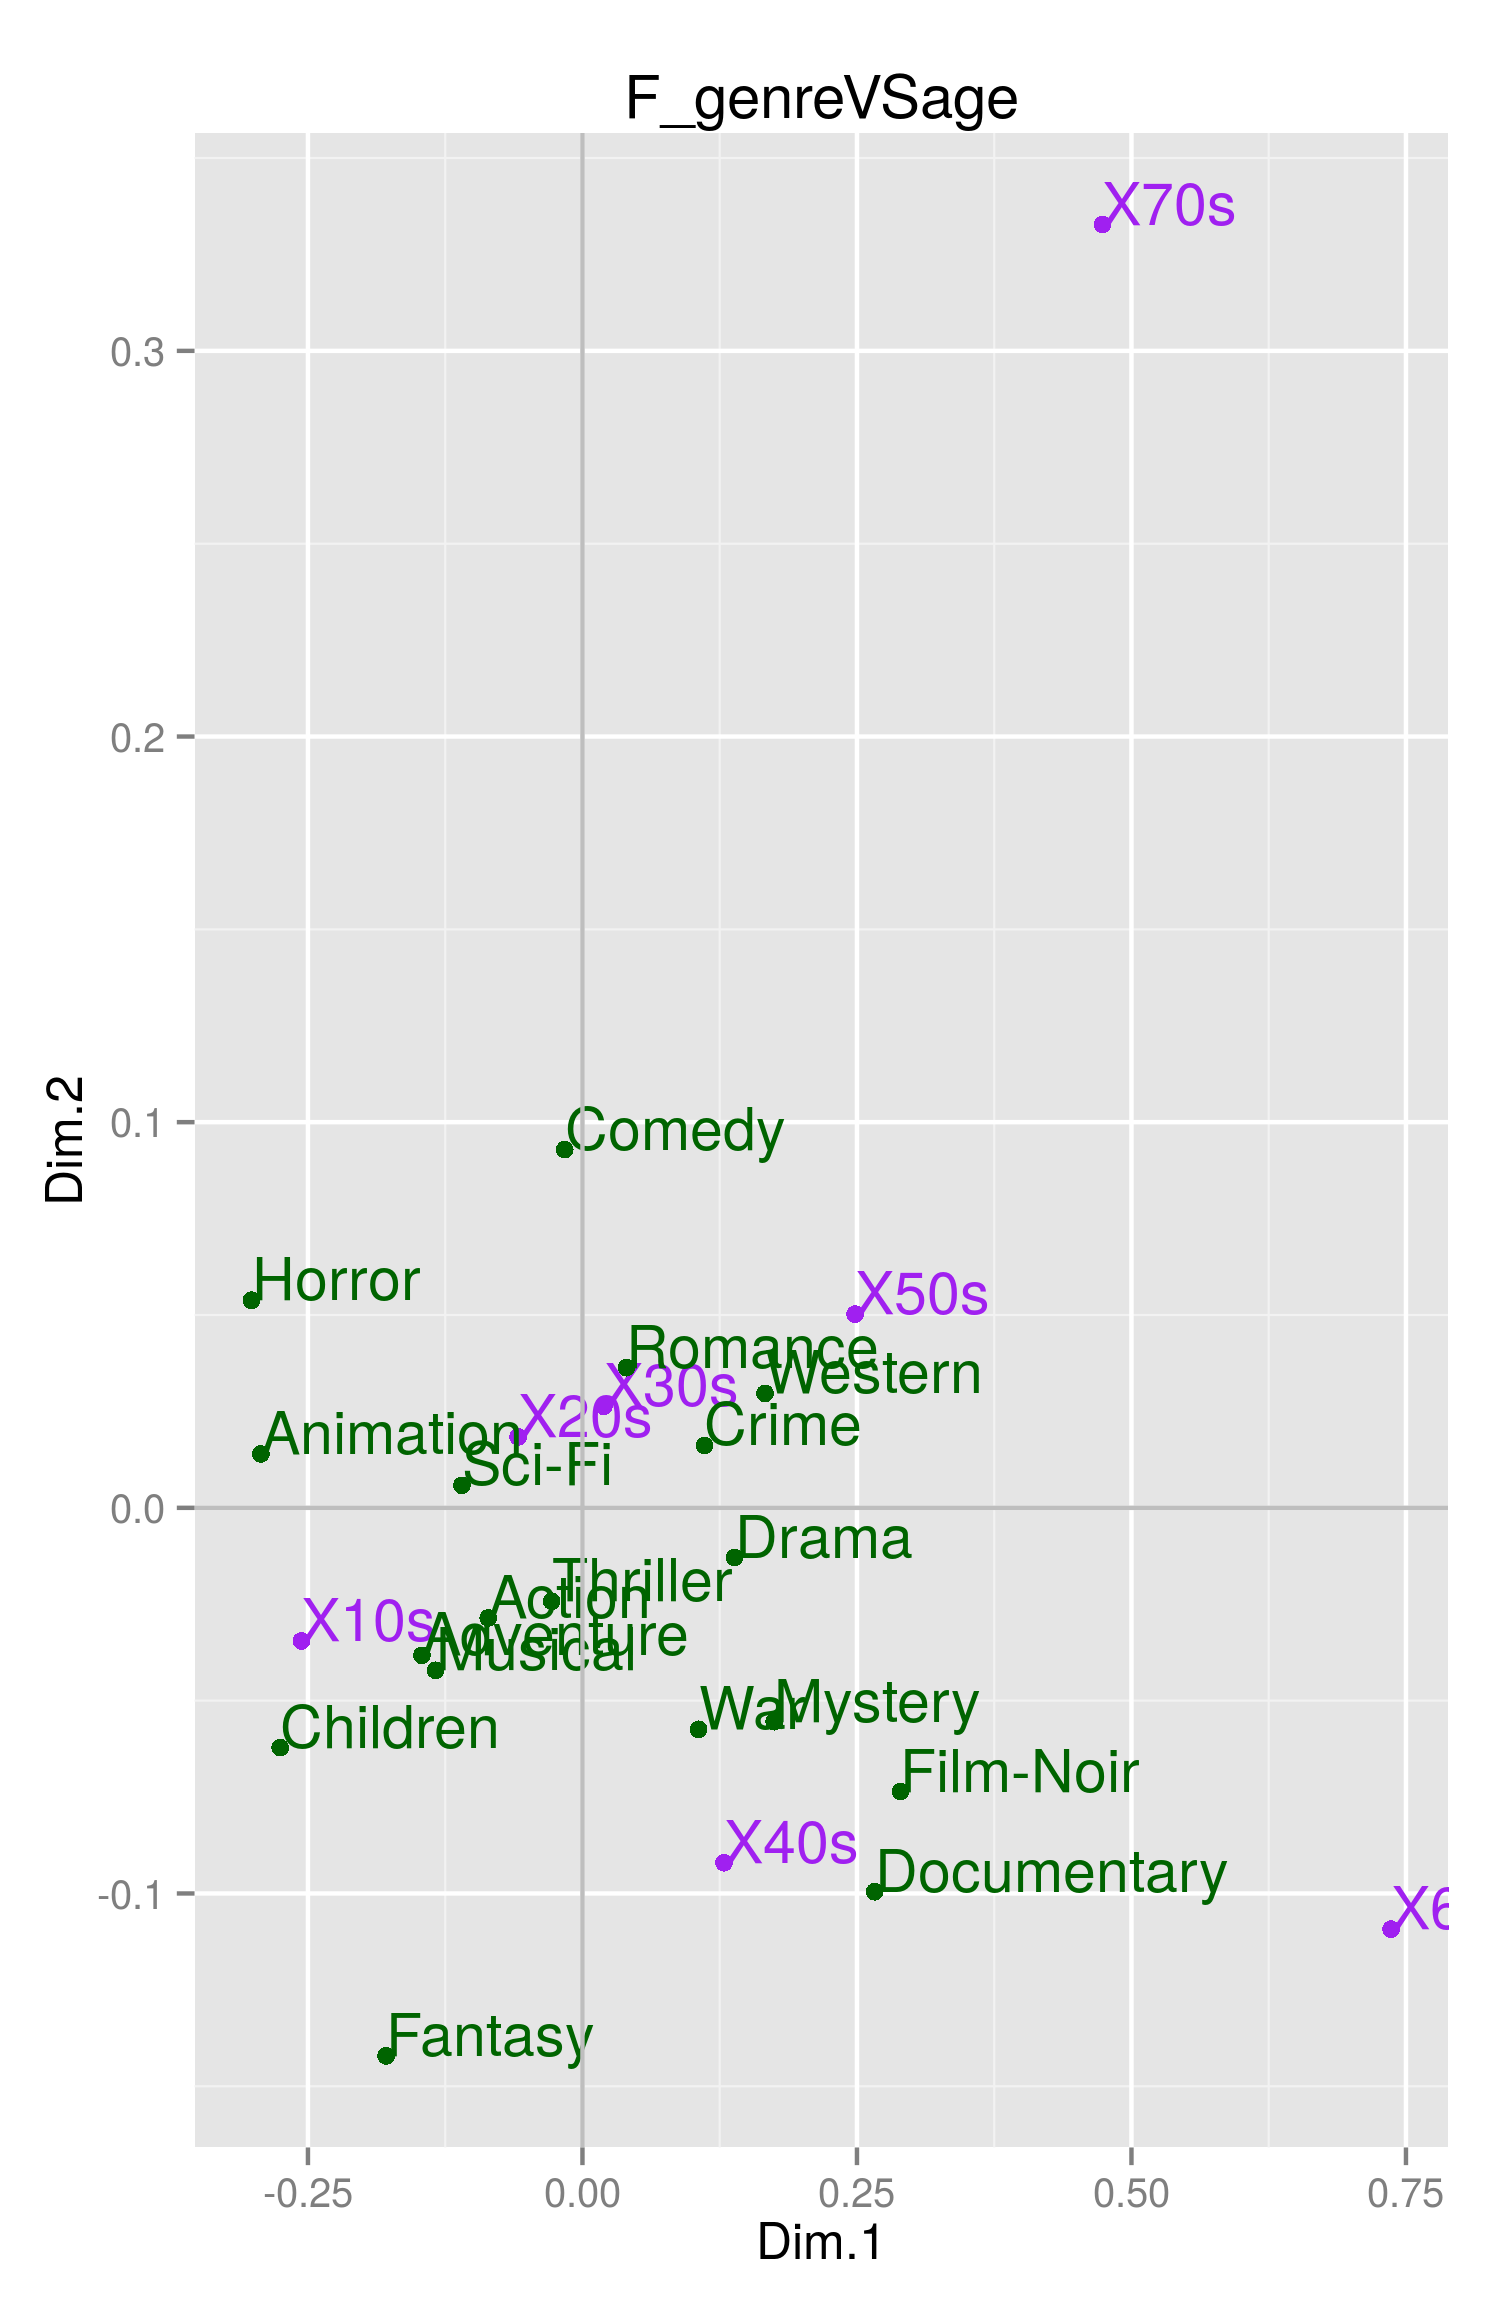
\includegraphics[scale=0.65]{./images/F_genreVSage}
\caption{Description des axes des AFC réalisées}
\end{figure}\bigskip
\


\pagebreak
\subsection{Hommes}
\begin{figure}[htd]
\centering
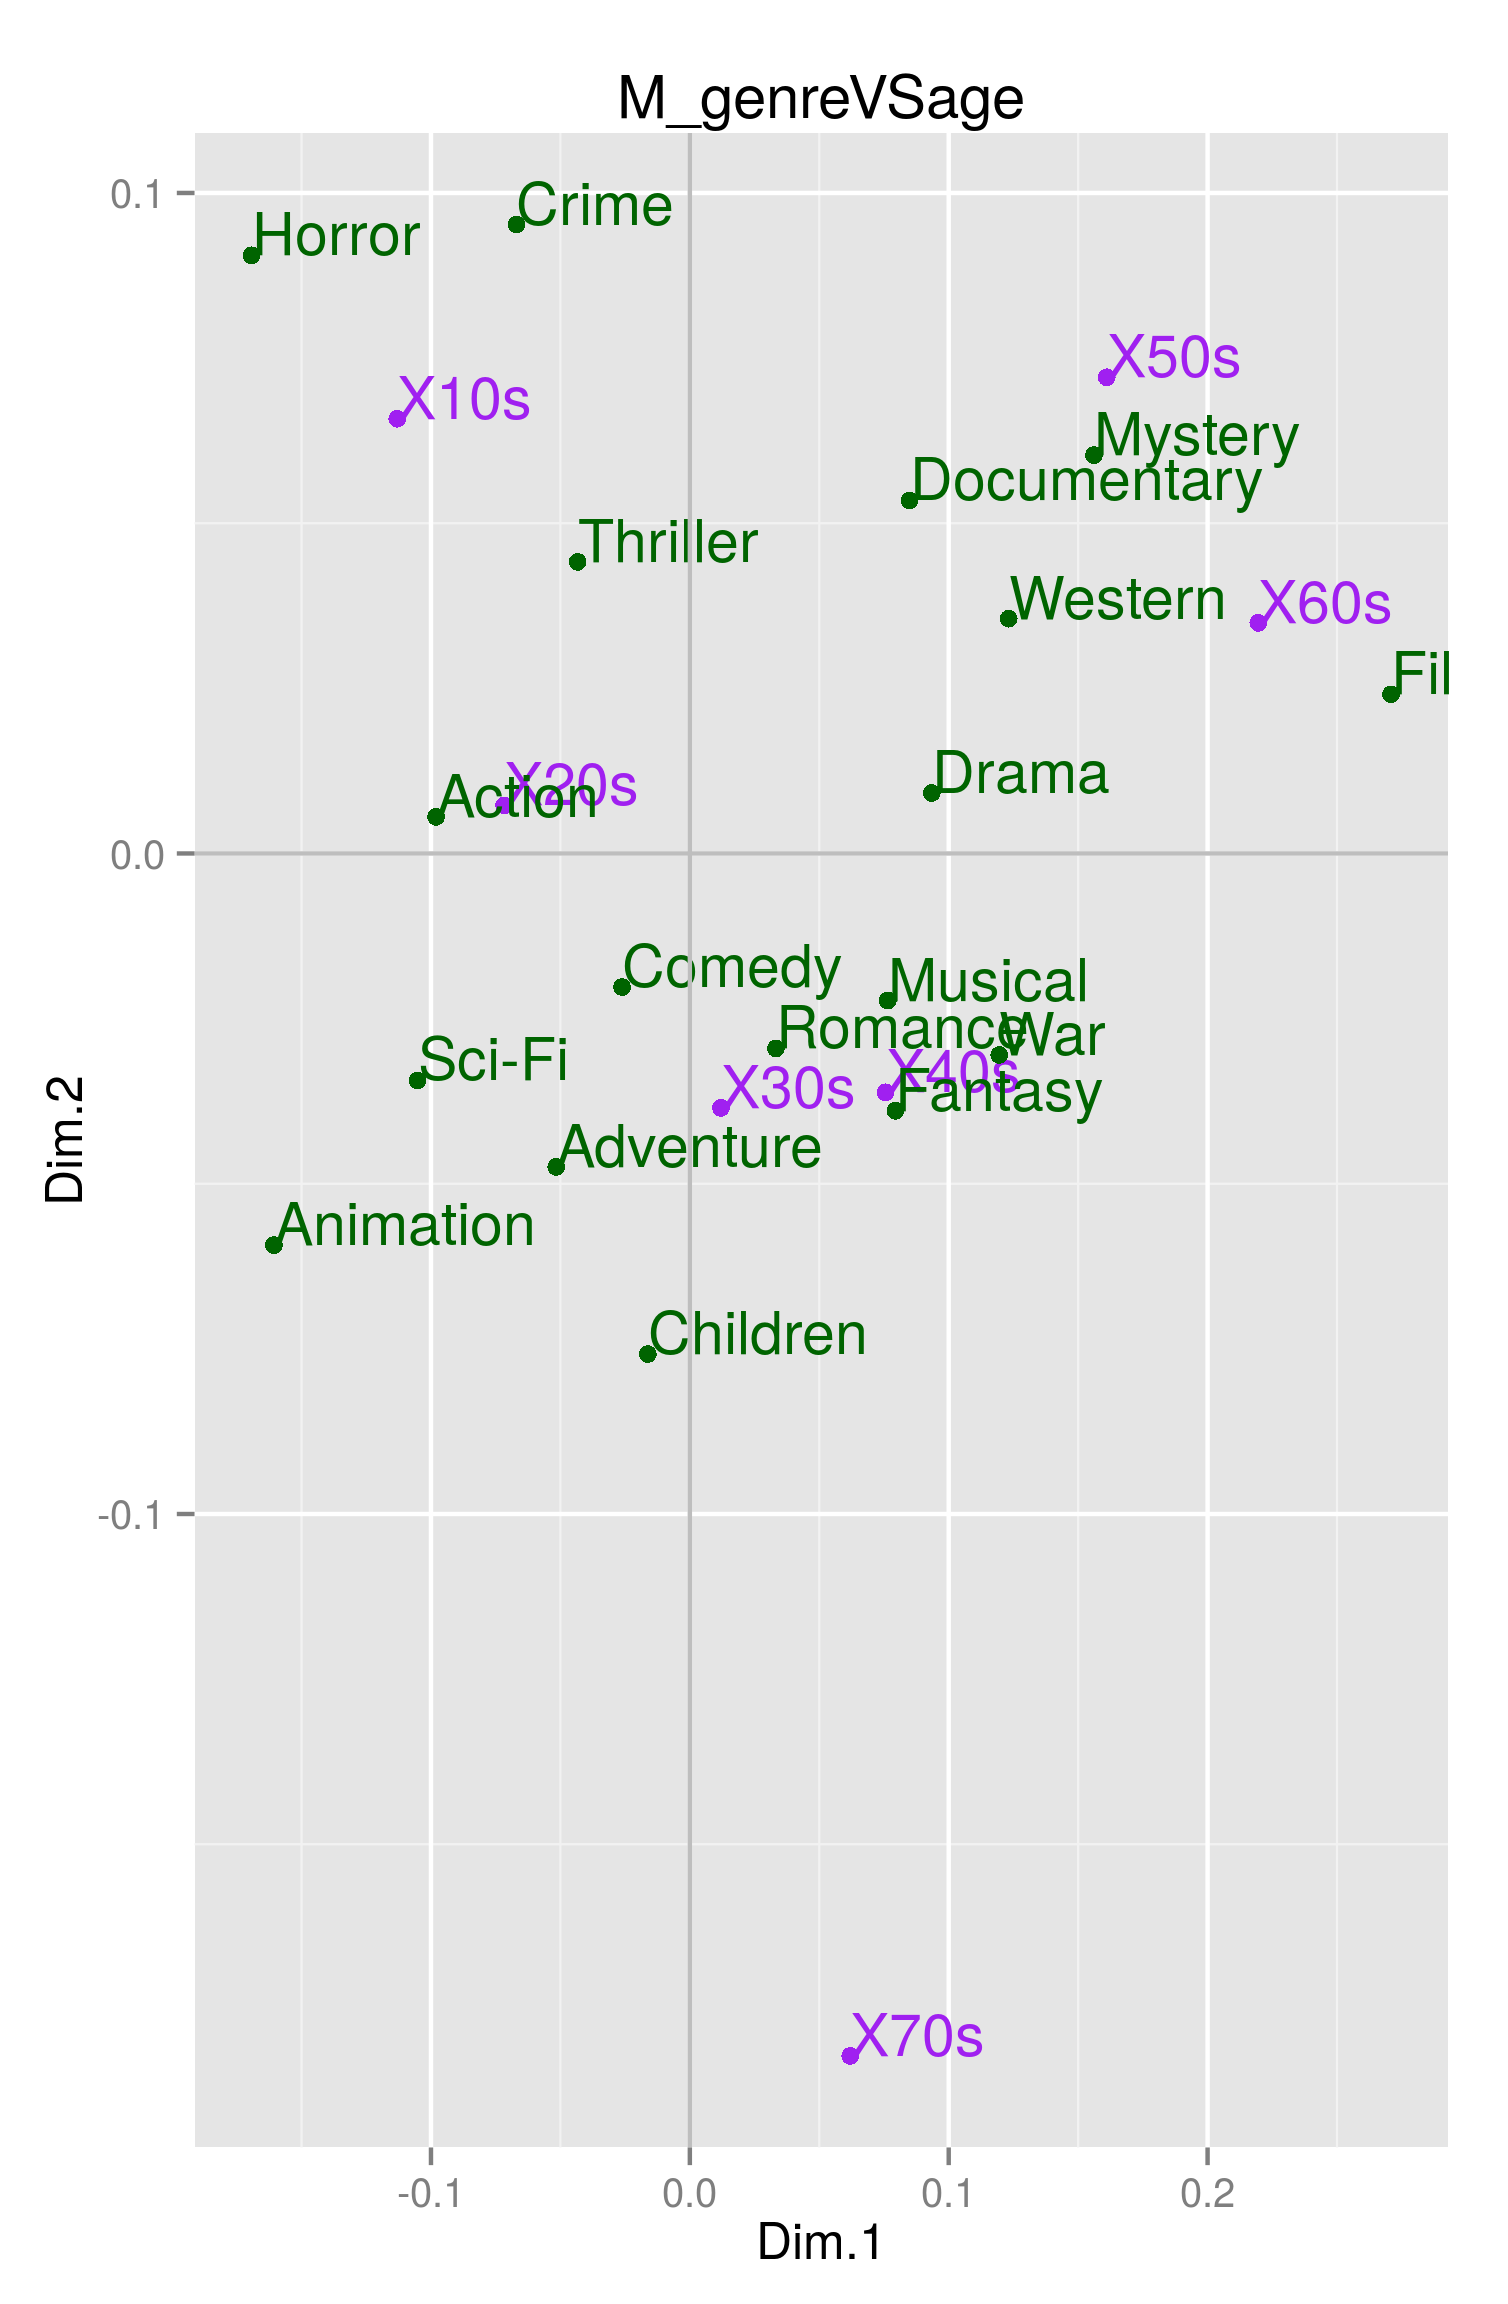
\includegraphics[scale=0.65]{./images/M_genreVSage}
\caption{Genres des films par rapport à l'âge des utilisateurs}
\end{figure}

\pagebreak
\section{Genre(s) des films | Occupation professionnelle des utilisateurs}
\subsection{Femmes}
\begin{figure}[htd]
\centering
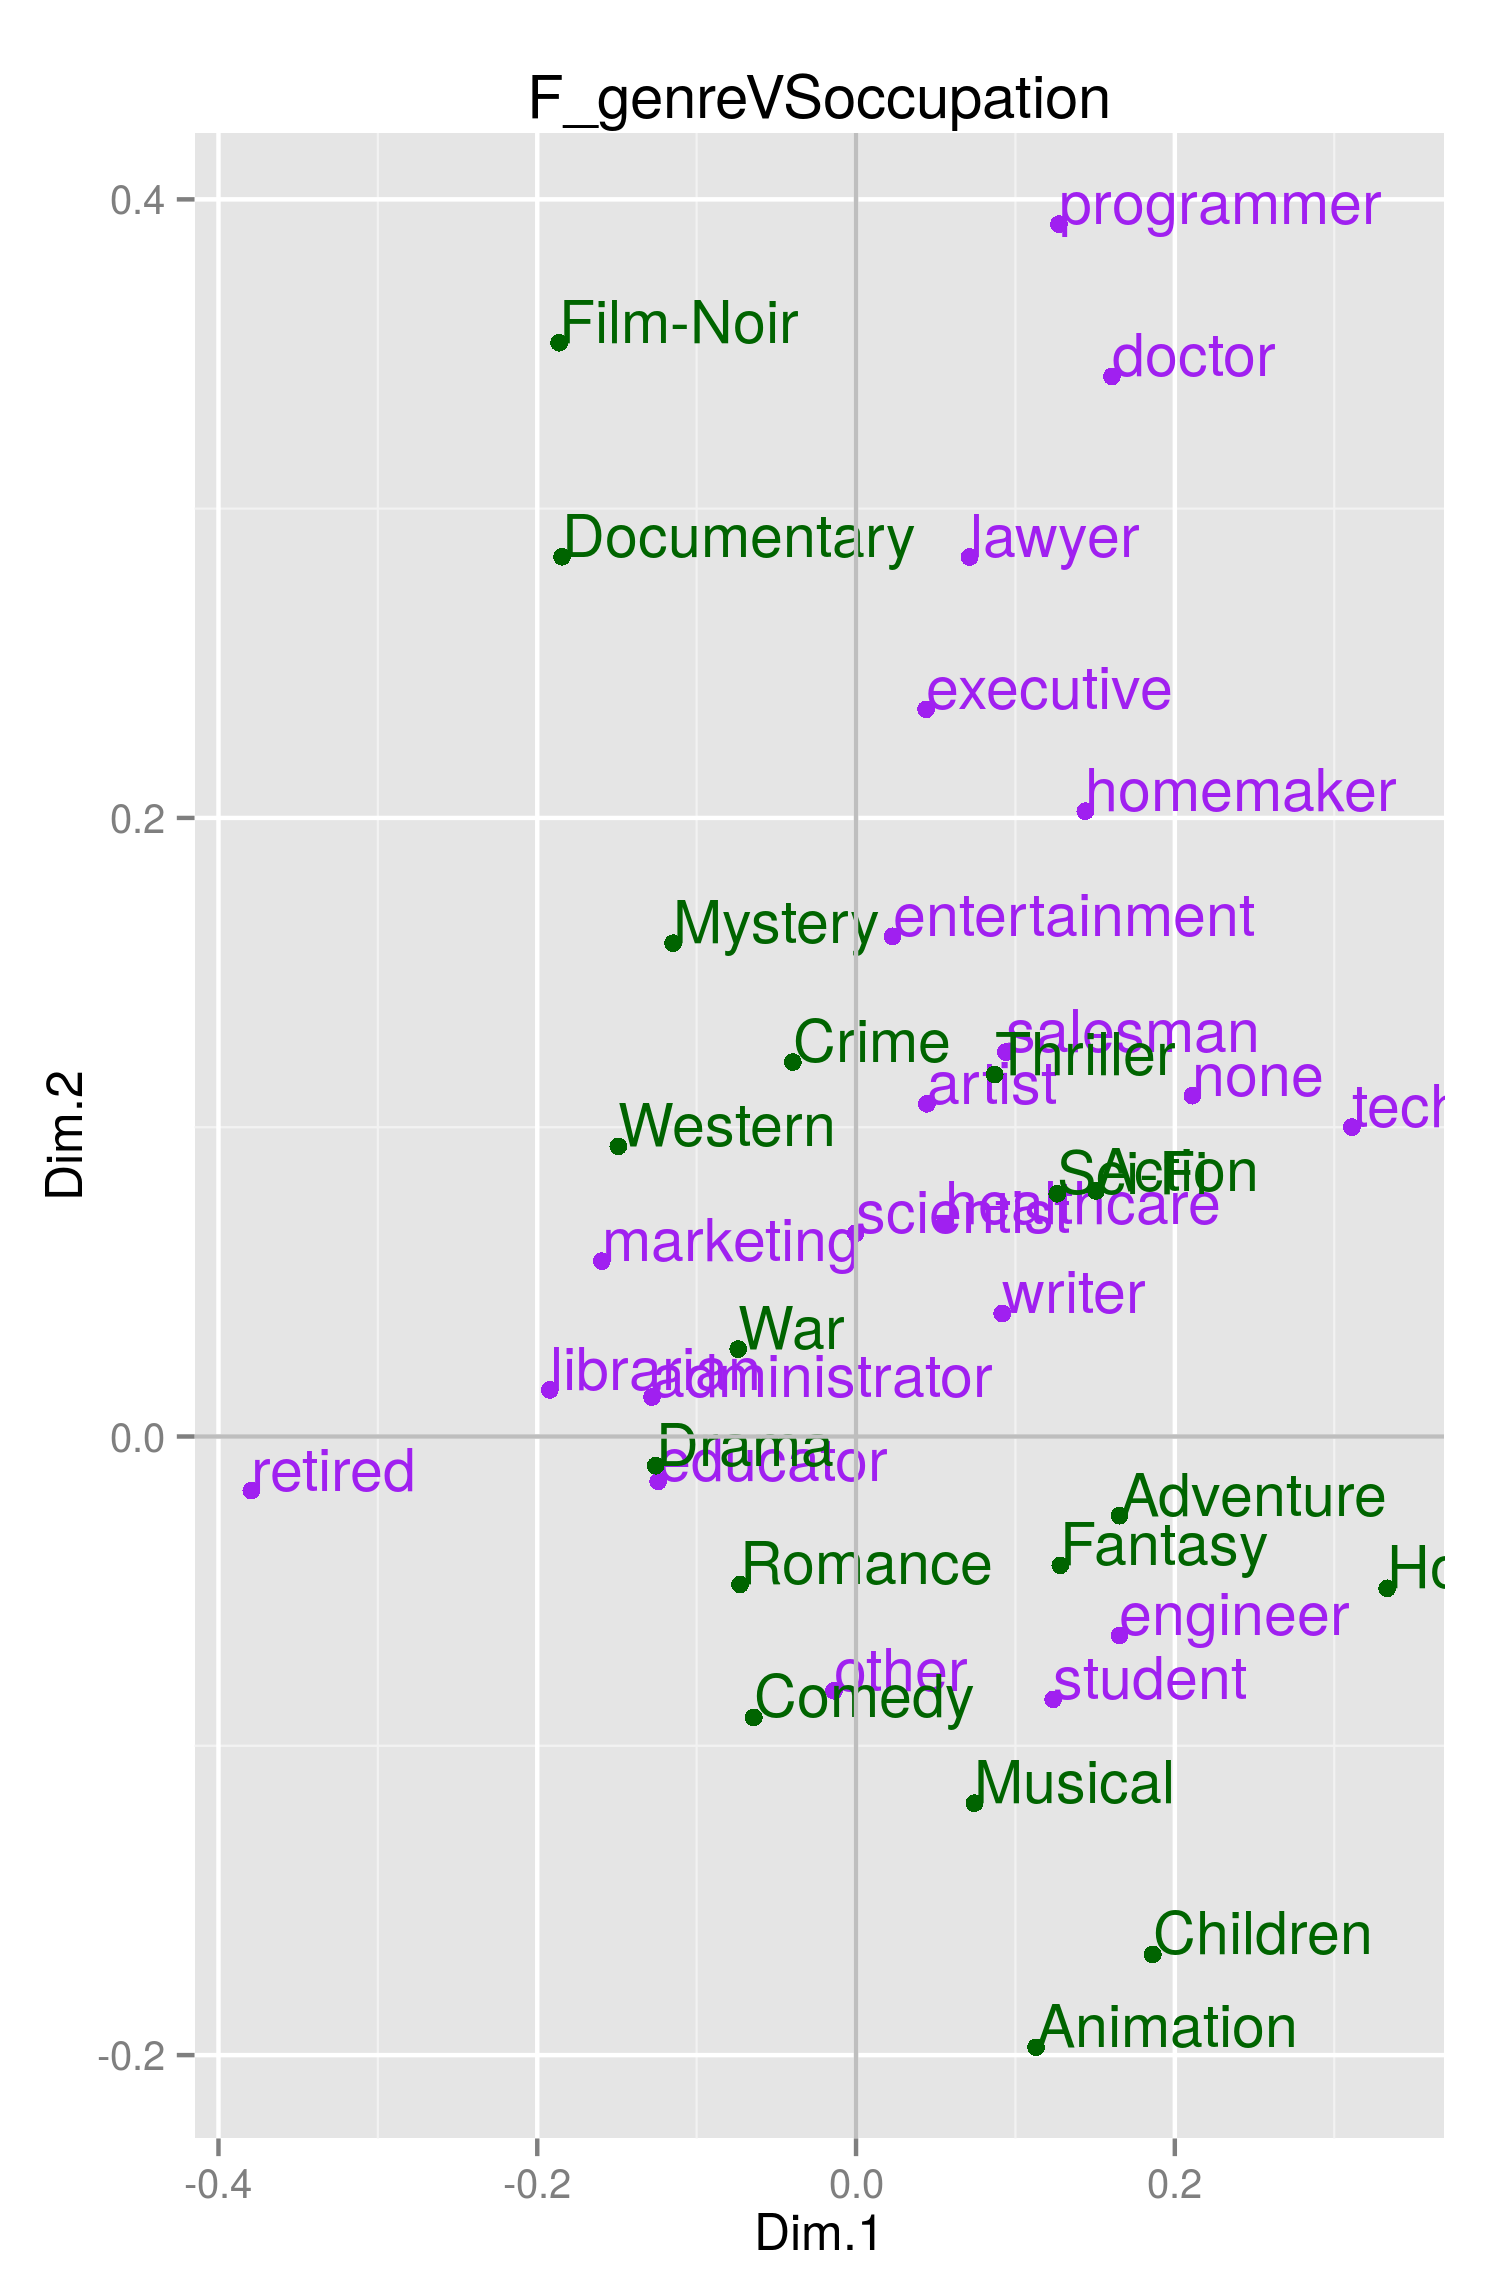
\includegraphics[scale=0.65]{./images/F_genreVSoccupation}
\caption{Genres des films par rapport à l'occupation professionnelle des utilisatrices}
\end{figure}

\pagebreak
\subsection{Hommes}
\begin{figure}[htd]
\centering
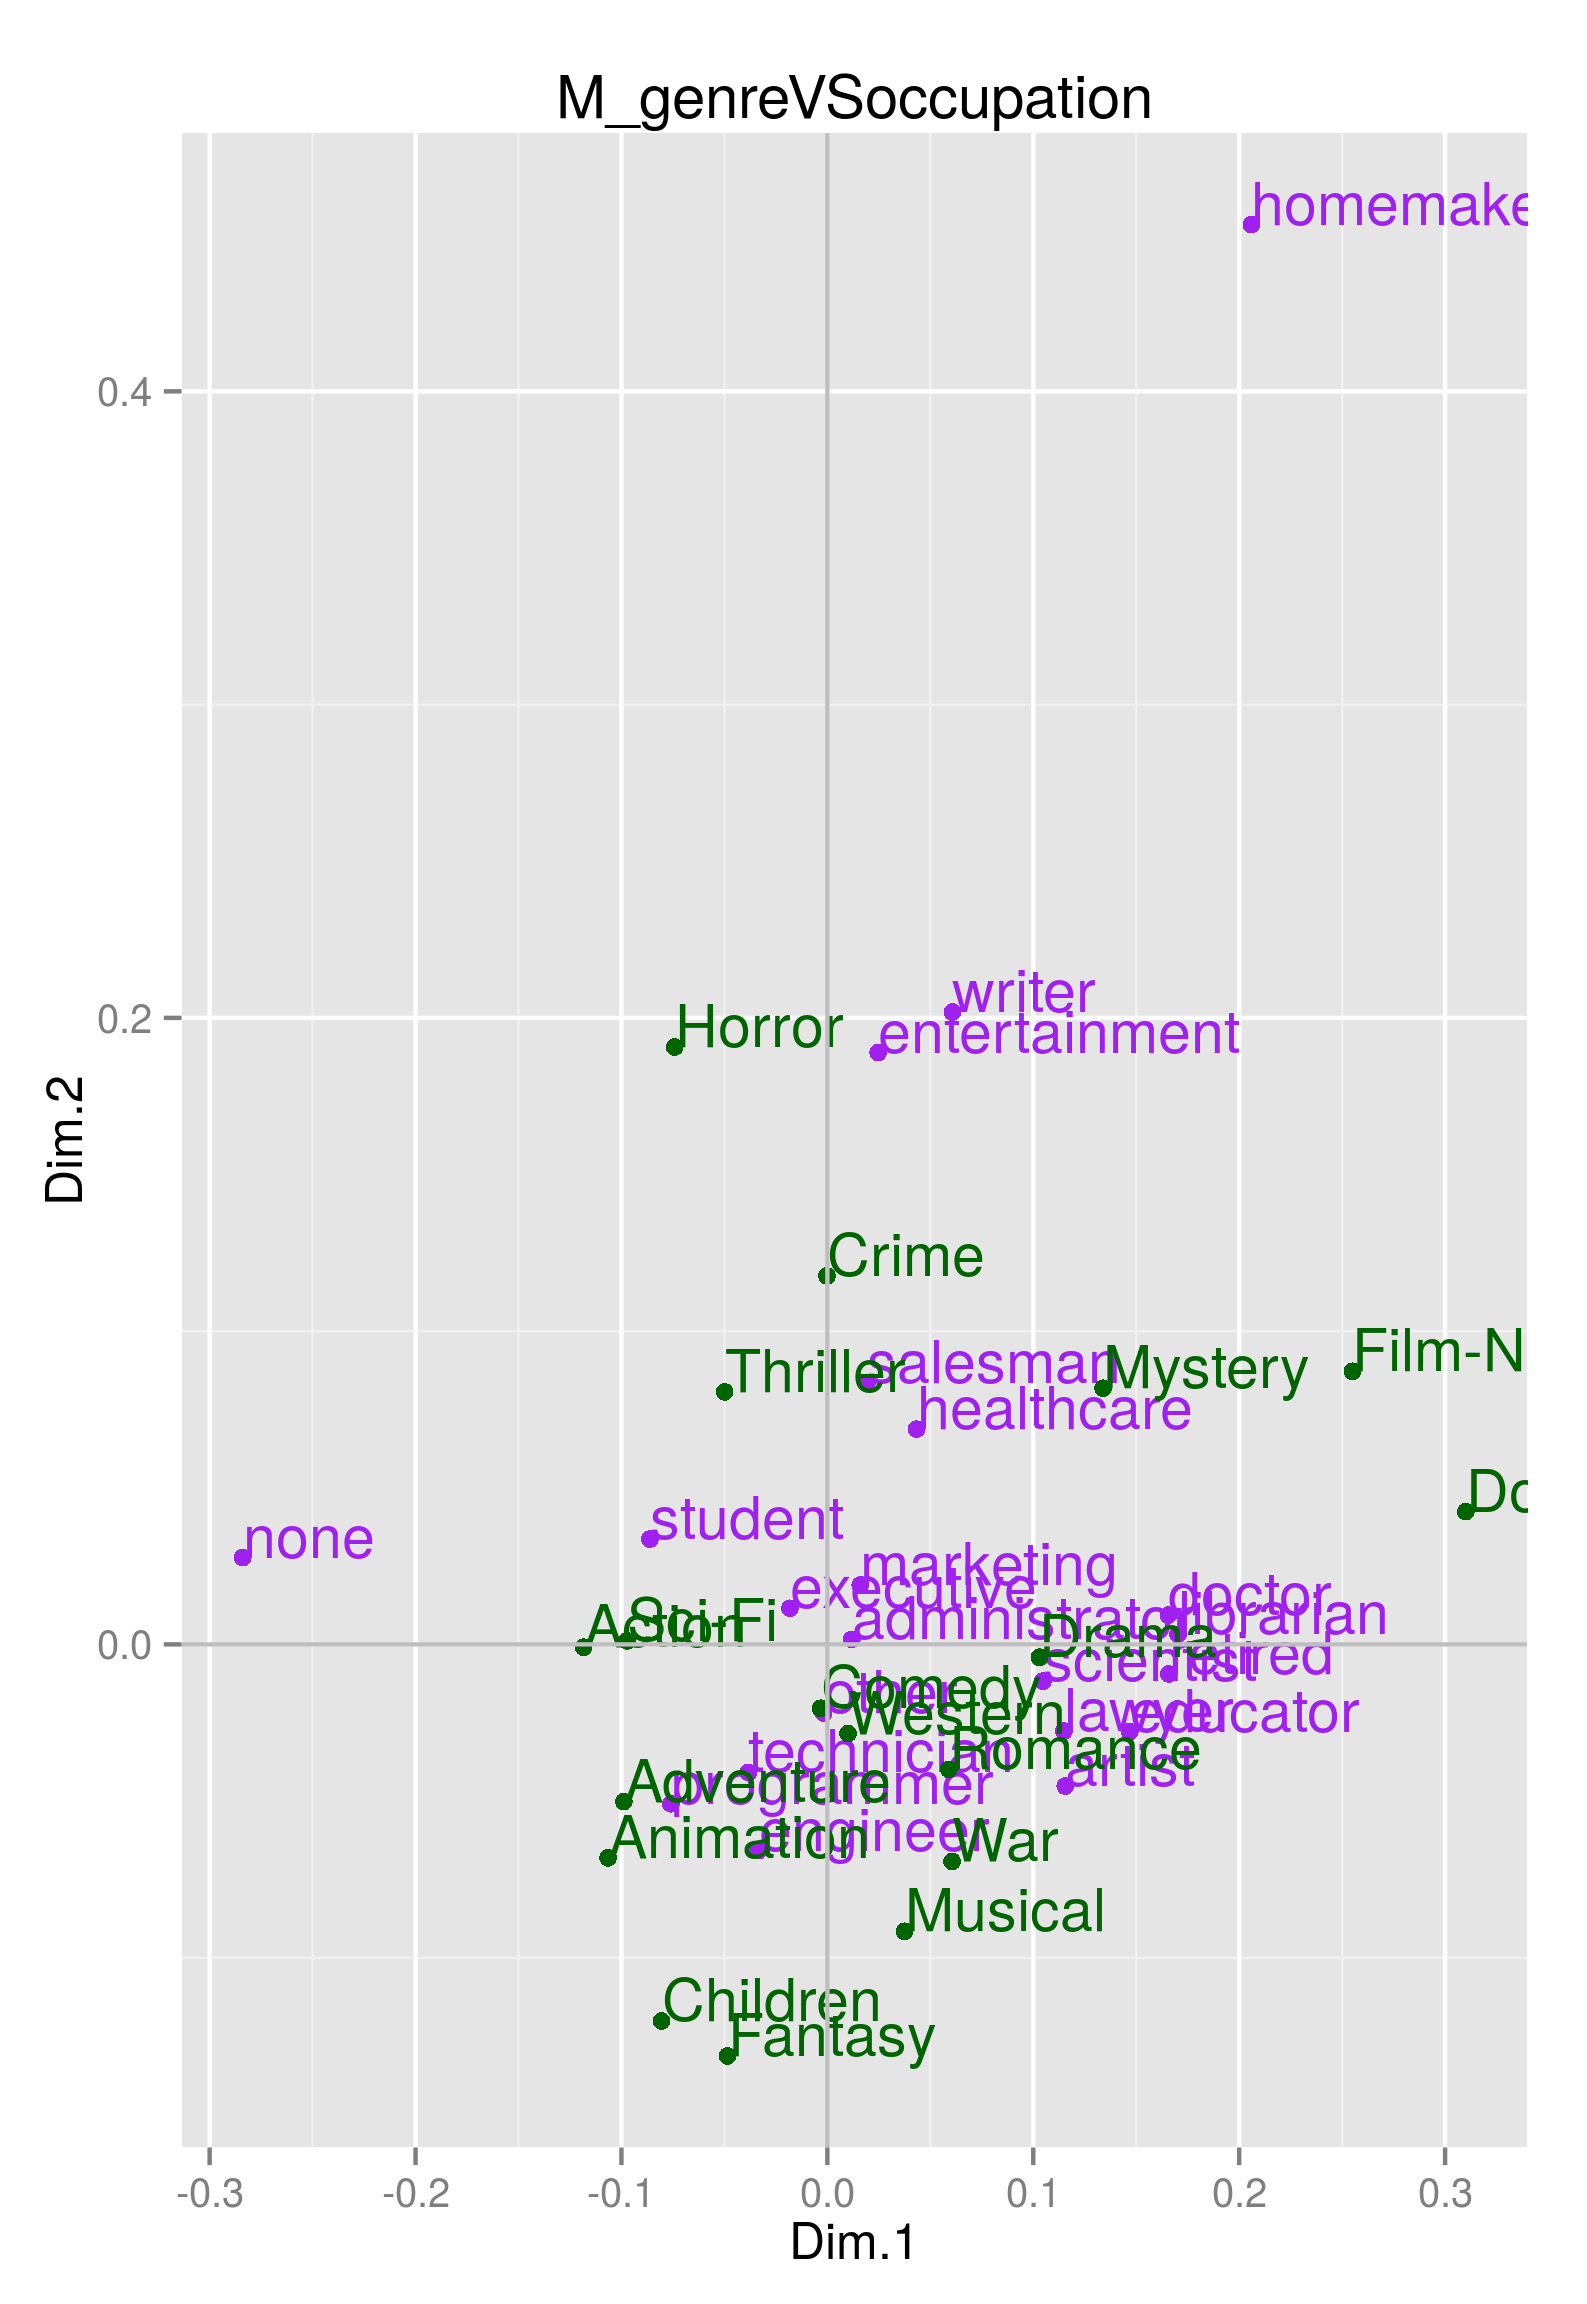
\includegraphics[scale=0.65]{./images/M_genreVSoccupation}
\caption{Genres des films par rapport à l'occupation professionnelle des utilisateurs}
\end{figure}


\pagebreak
\section{Genre(s) des films | Région d'habitation des utilisateurs}
\subsection{Femmes}
\begin{figure}[htd]
\centering
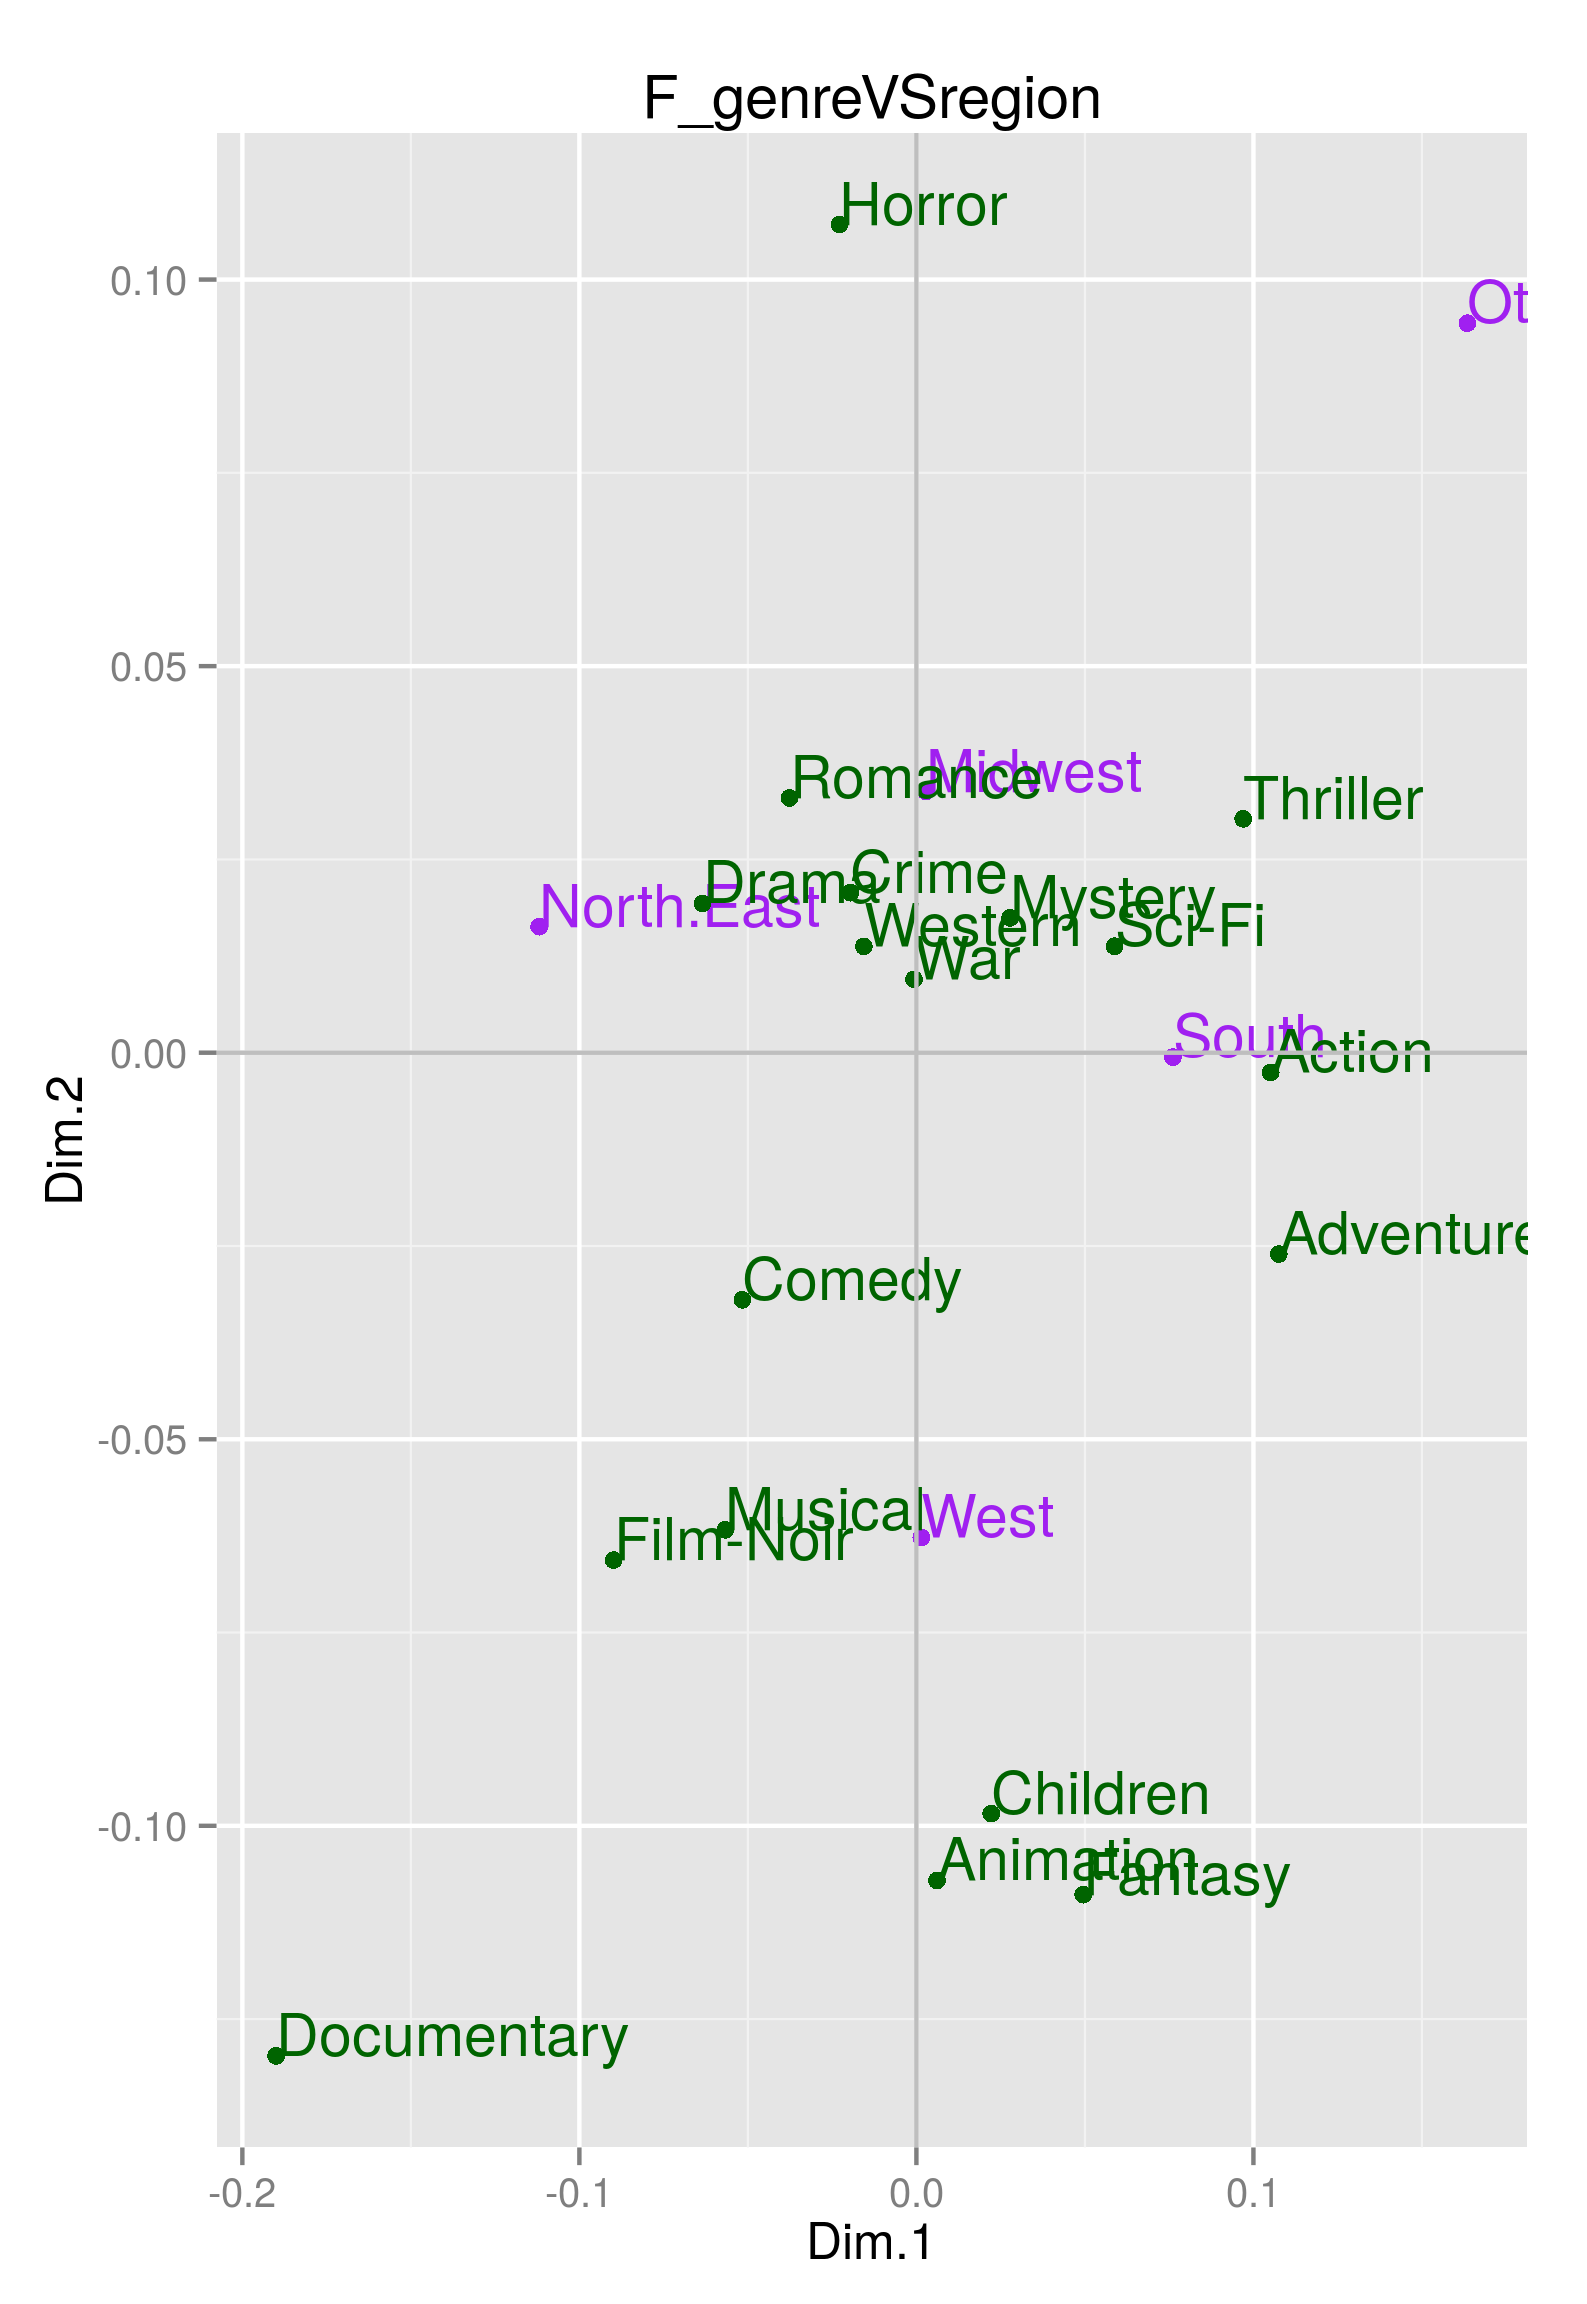
\includegraphics[scale=0.65]{./images/F_genreVSregion}
\caption{Genres des films par rapport à la région d'habitation des utilisatrices}
\end{figure}

\pagebreak
\subsection{Hommes}
\begin{figure}[htd]
\centering
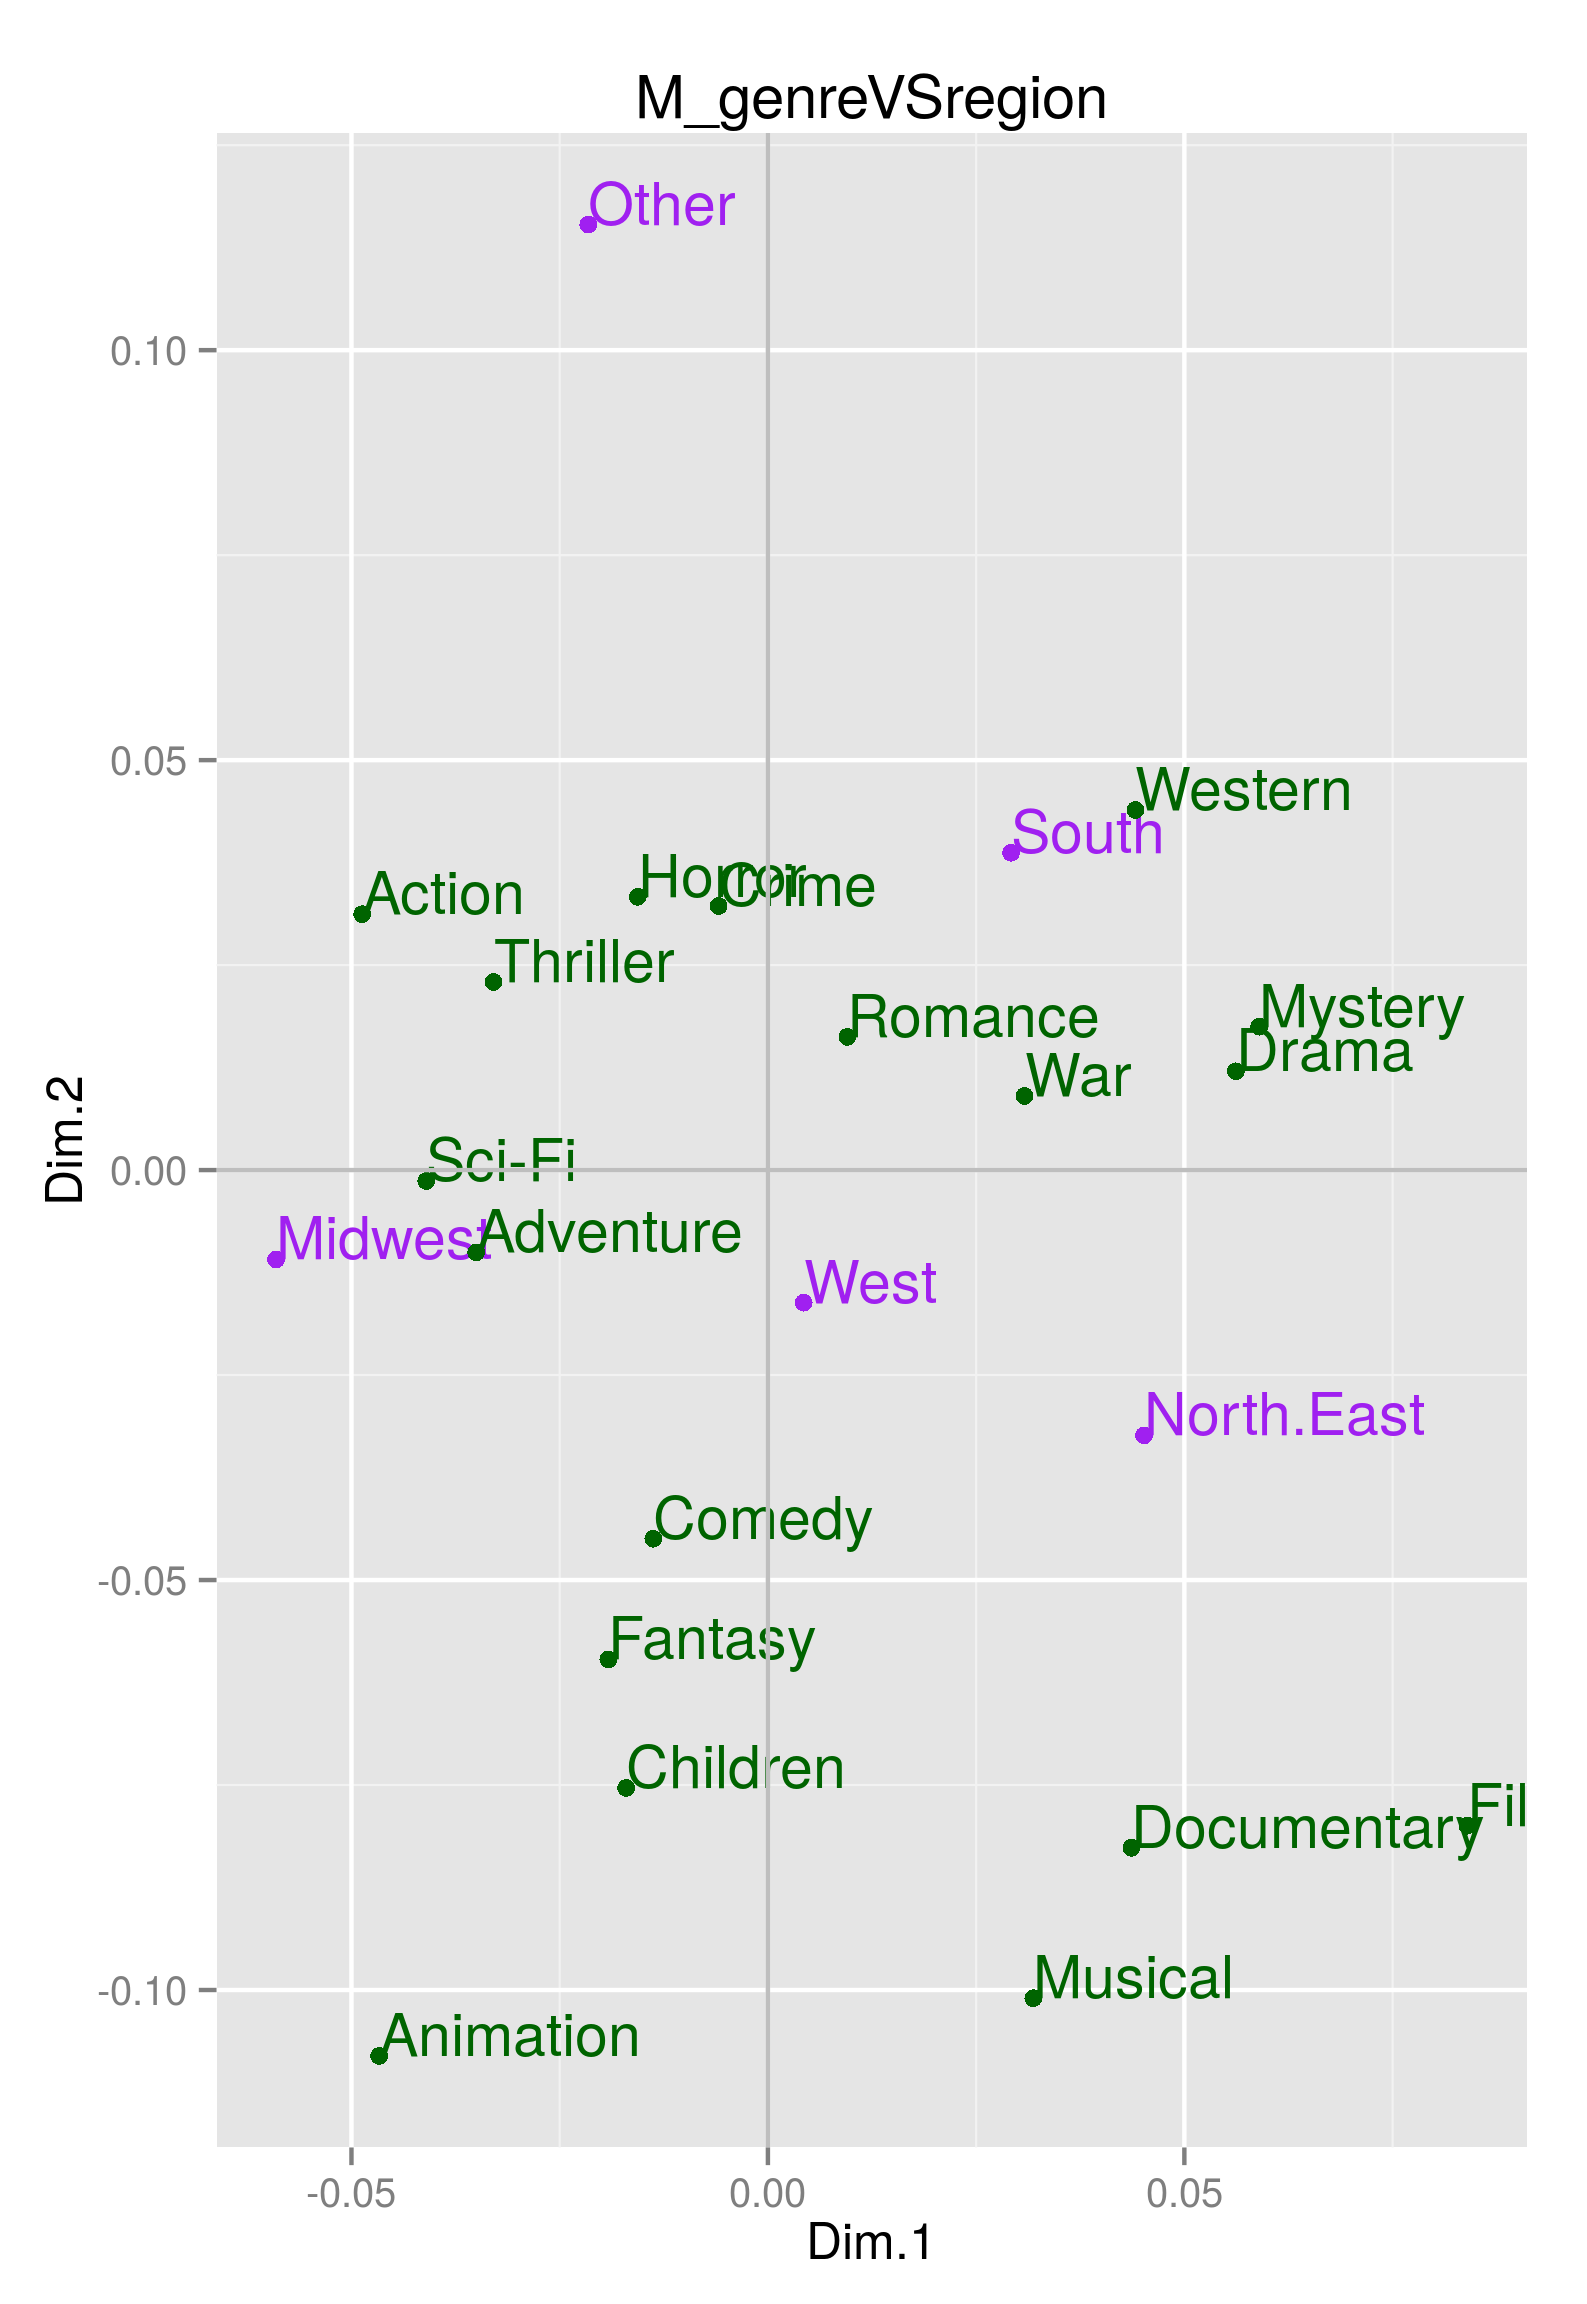
\includegraphics[scale=0.65]{./images/M_genreVSregion}
\caption{Genres des films par rapport à la région d'habitation des utilisateurs}
\end{figure}

\pagebreak
\section{Décennie de sortie des films | Catégorie d'âge des utilisateurs}
\subsection{Femmes}
\begin{figure}[htd]
\centering
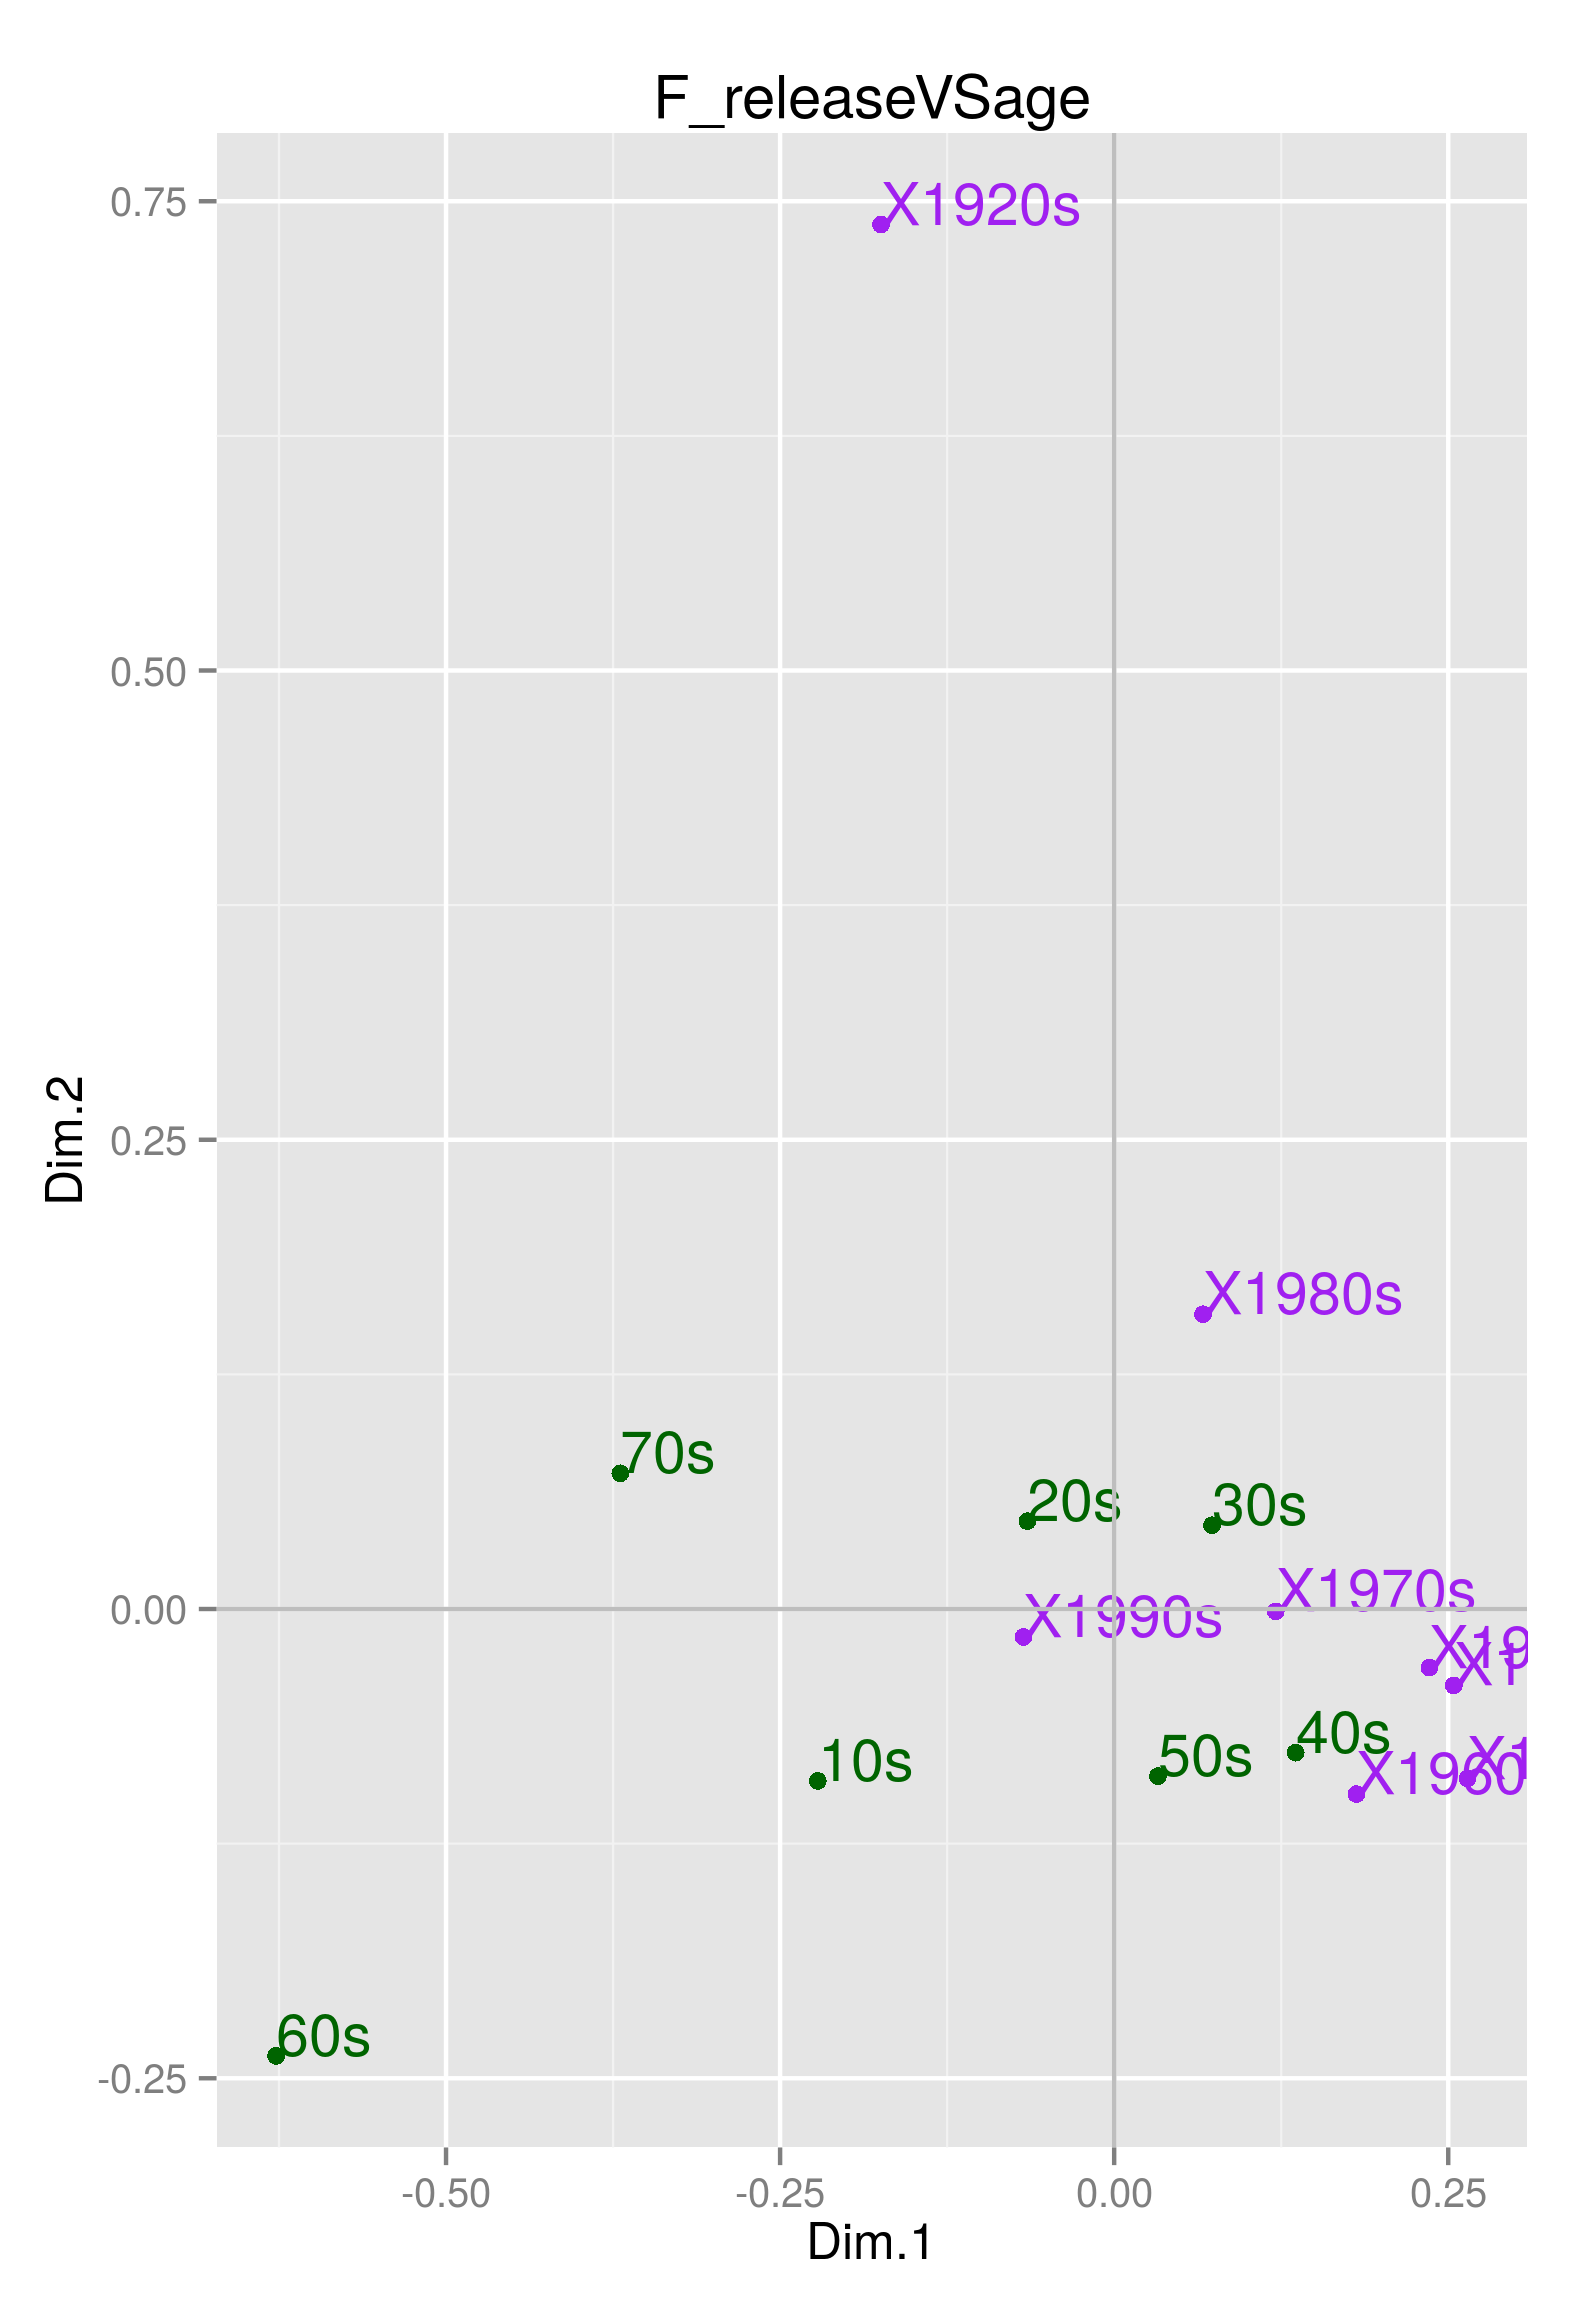
\includegraphics[scale=0.65]{./images/F_releaseVSage}
\caption{Décennie de sortie des films par rapport à l'âge des utilisatrices}
\end{figure}

\pagebreak
\subsection{Hommes}
\begin{figure}[htd]
\centering
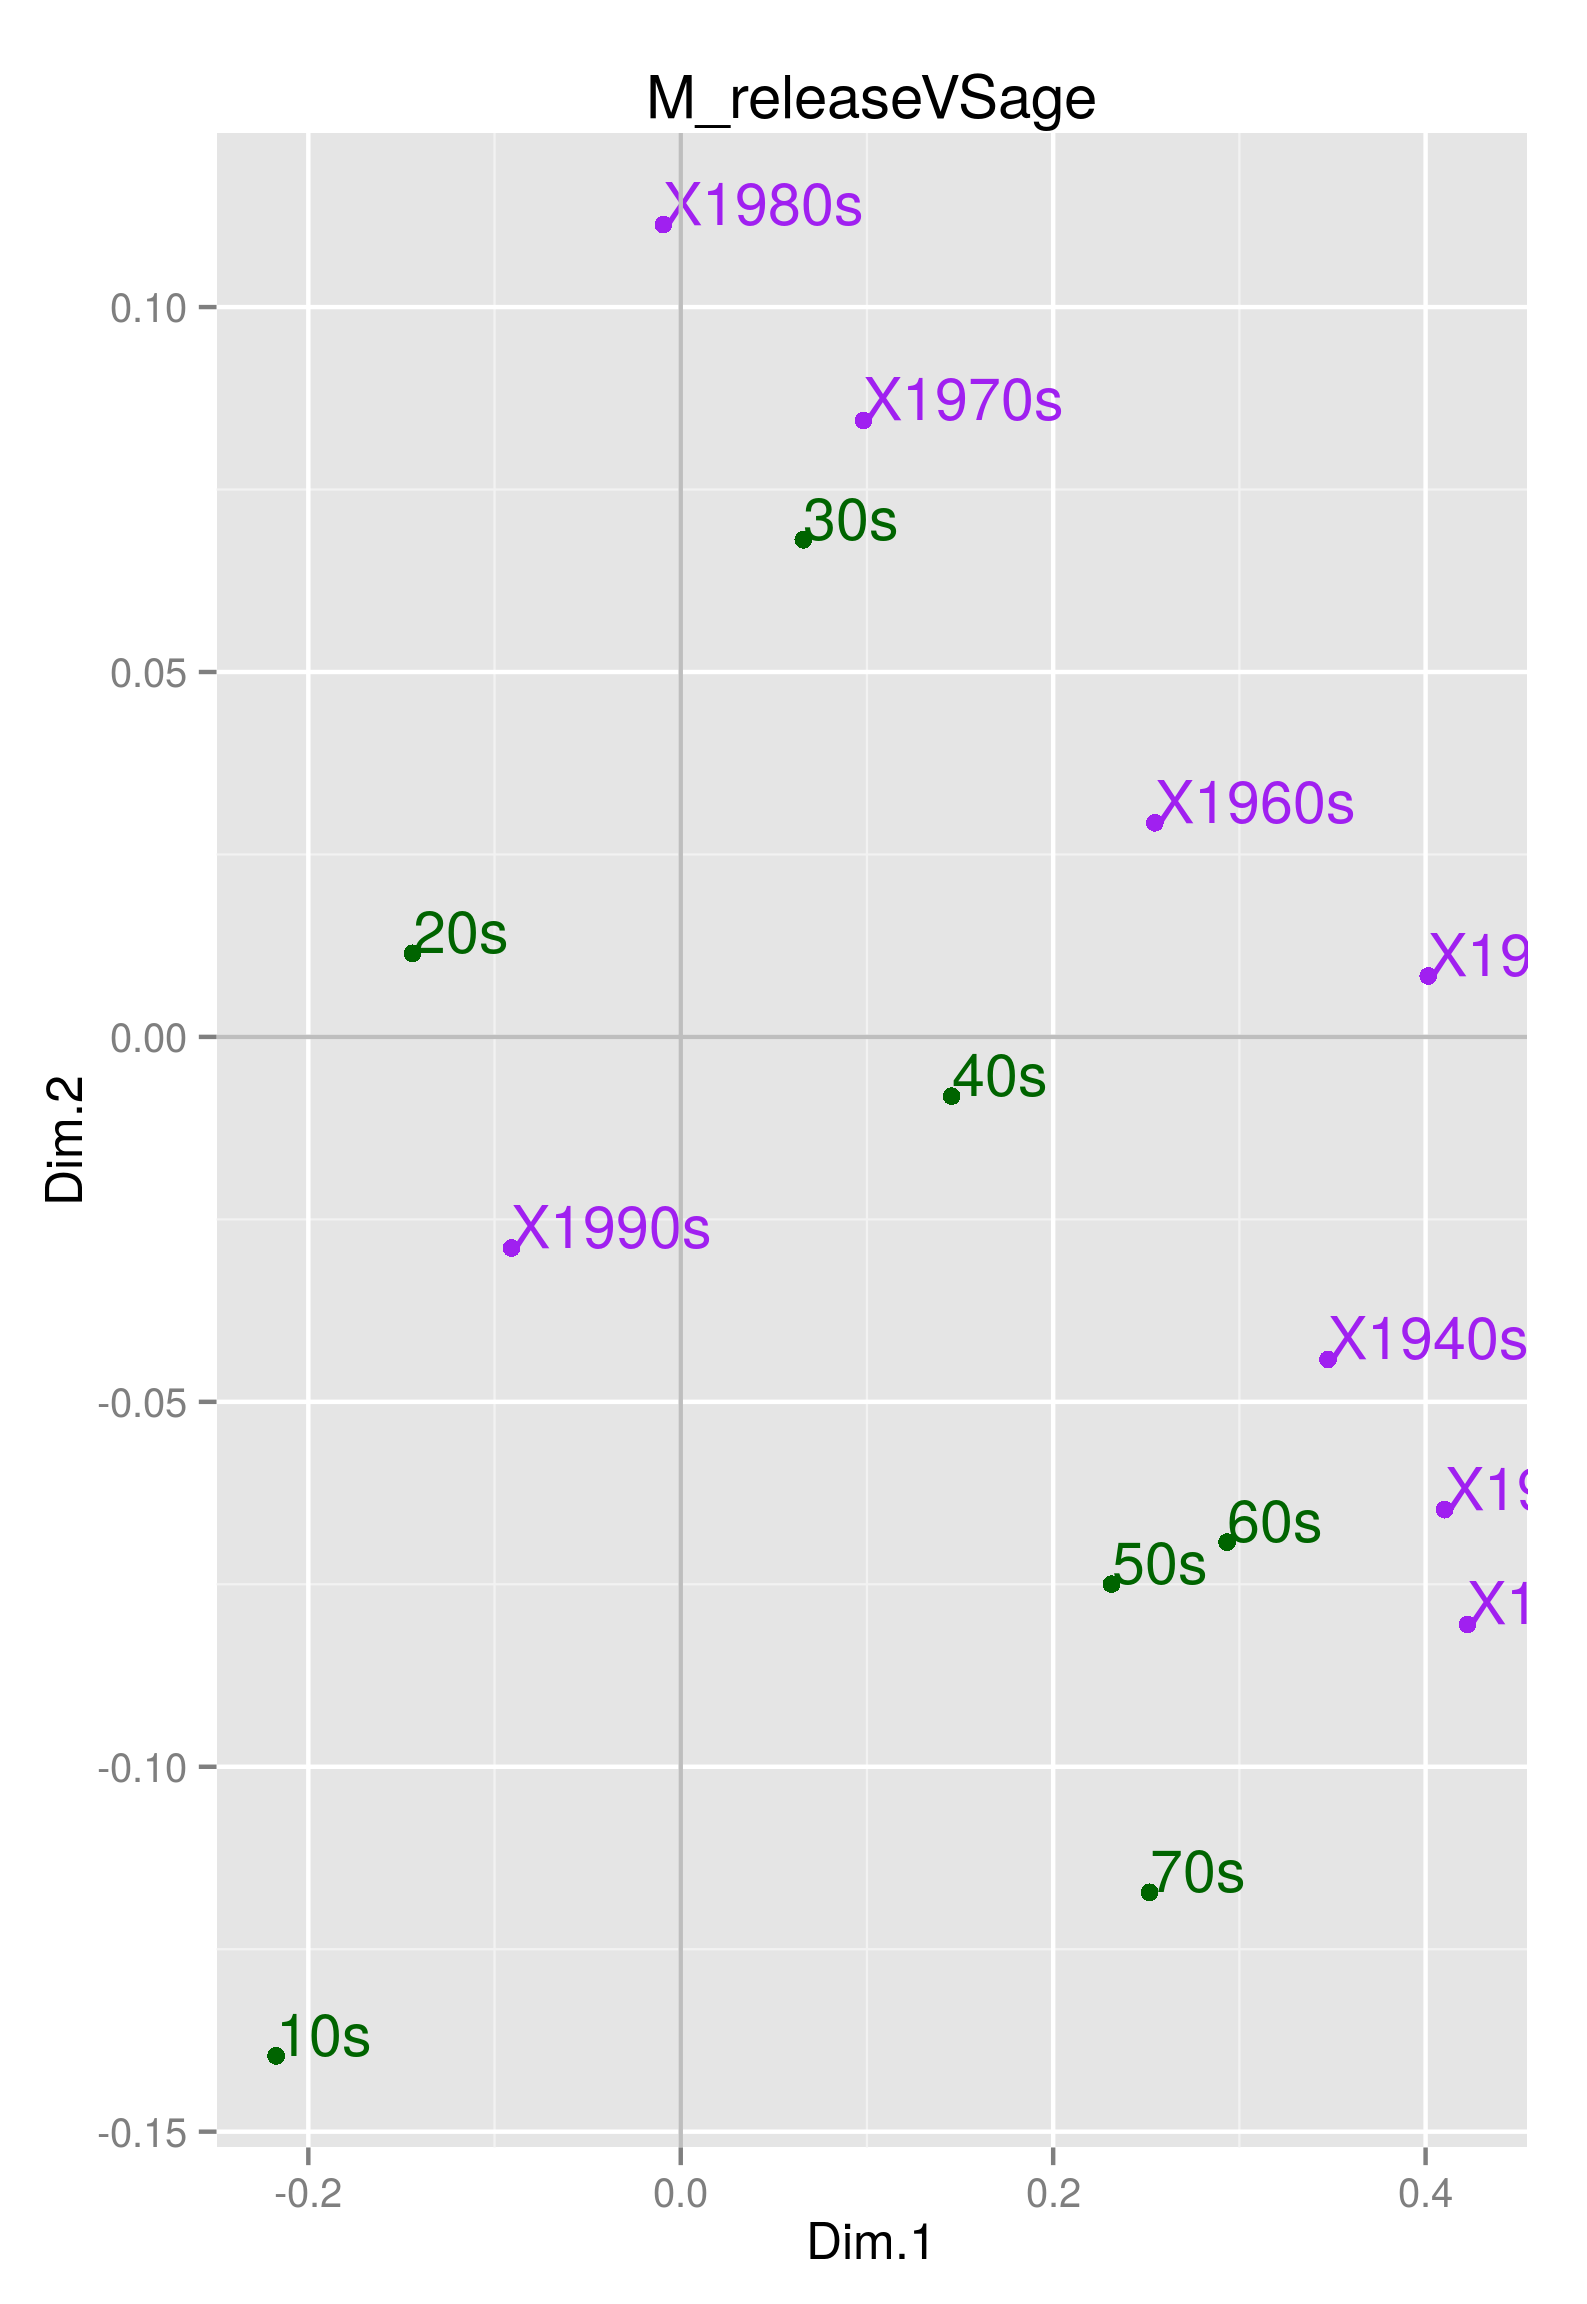
\includegraphics[scale=0.65]{./images/M_releaseVSage}
\caption{Décennie de sortie des films par rapport à l'âge des utilisateurs}
\end{figure}

\pagebreak
\section{Décennie de sortie des films | Occupation professionnelle des utilisateurs}
\subsection{Femmes}
\begin{figure}[htd]
\centering
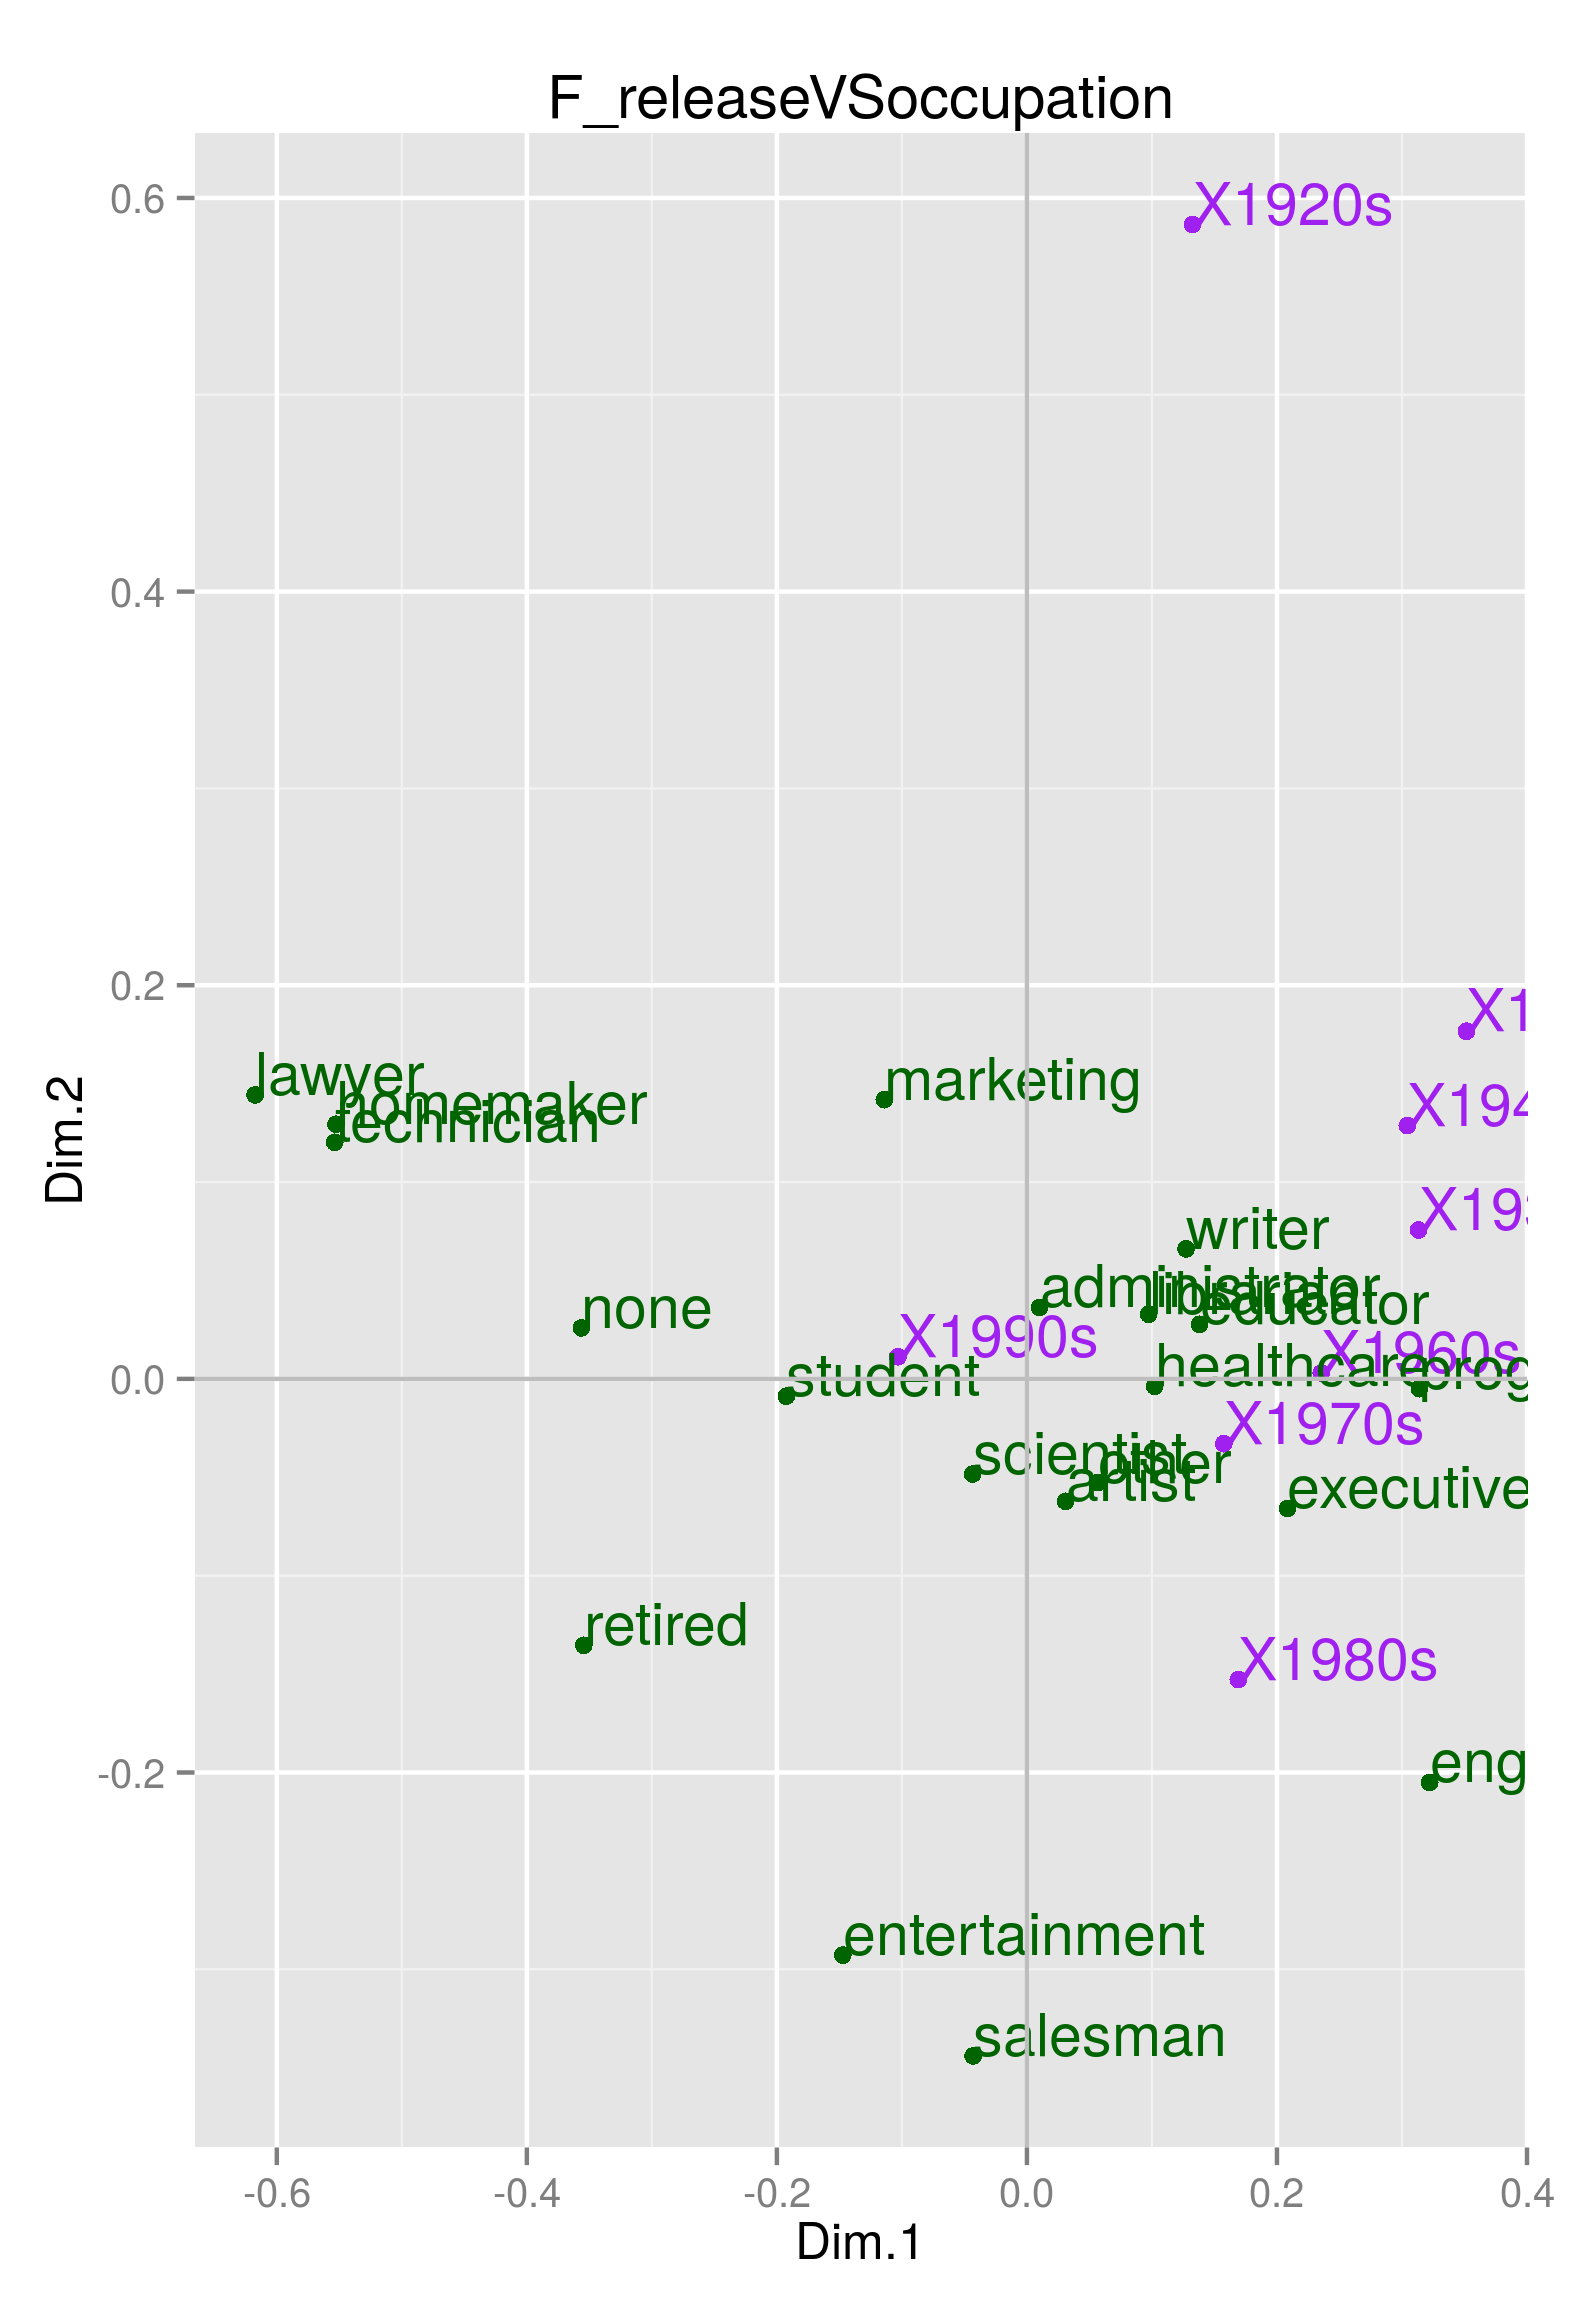
\includegraphics[scale=0.65]{./images/F_releaseVSoccupation}
\caption{Décennie de sortie des films par rapport à l'occupation professionnelle des utilisatrices}
\end{figure}

\pagebreak
\subsection{Hommes}
\begin{figure}[htd]
\centering
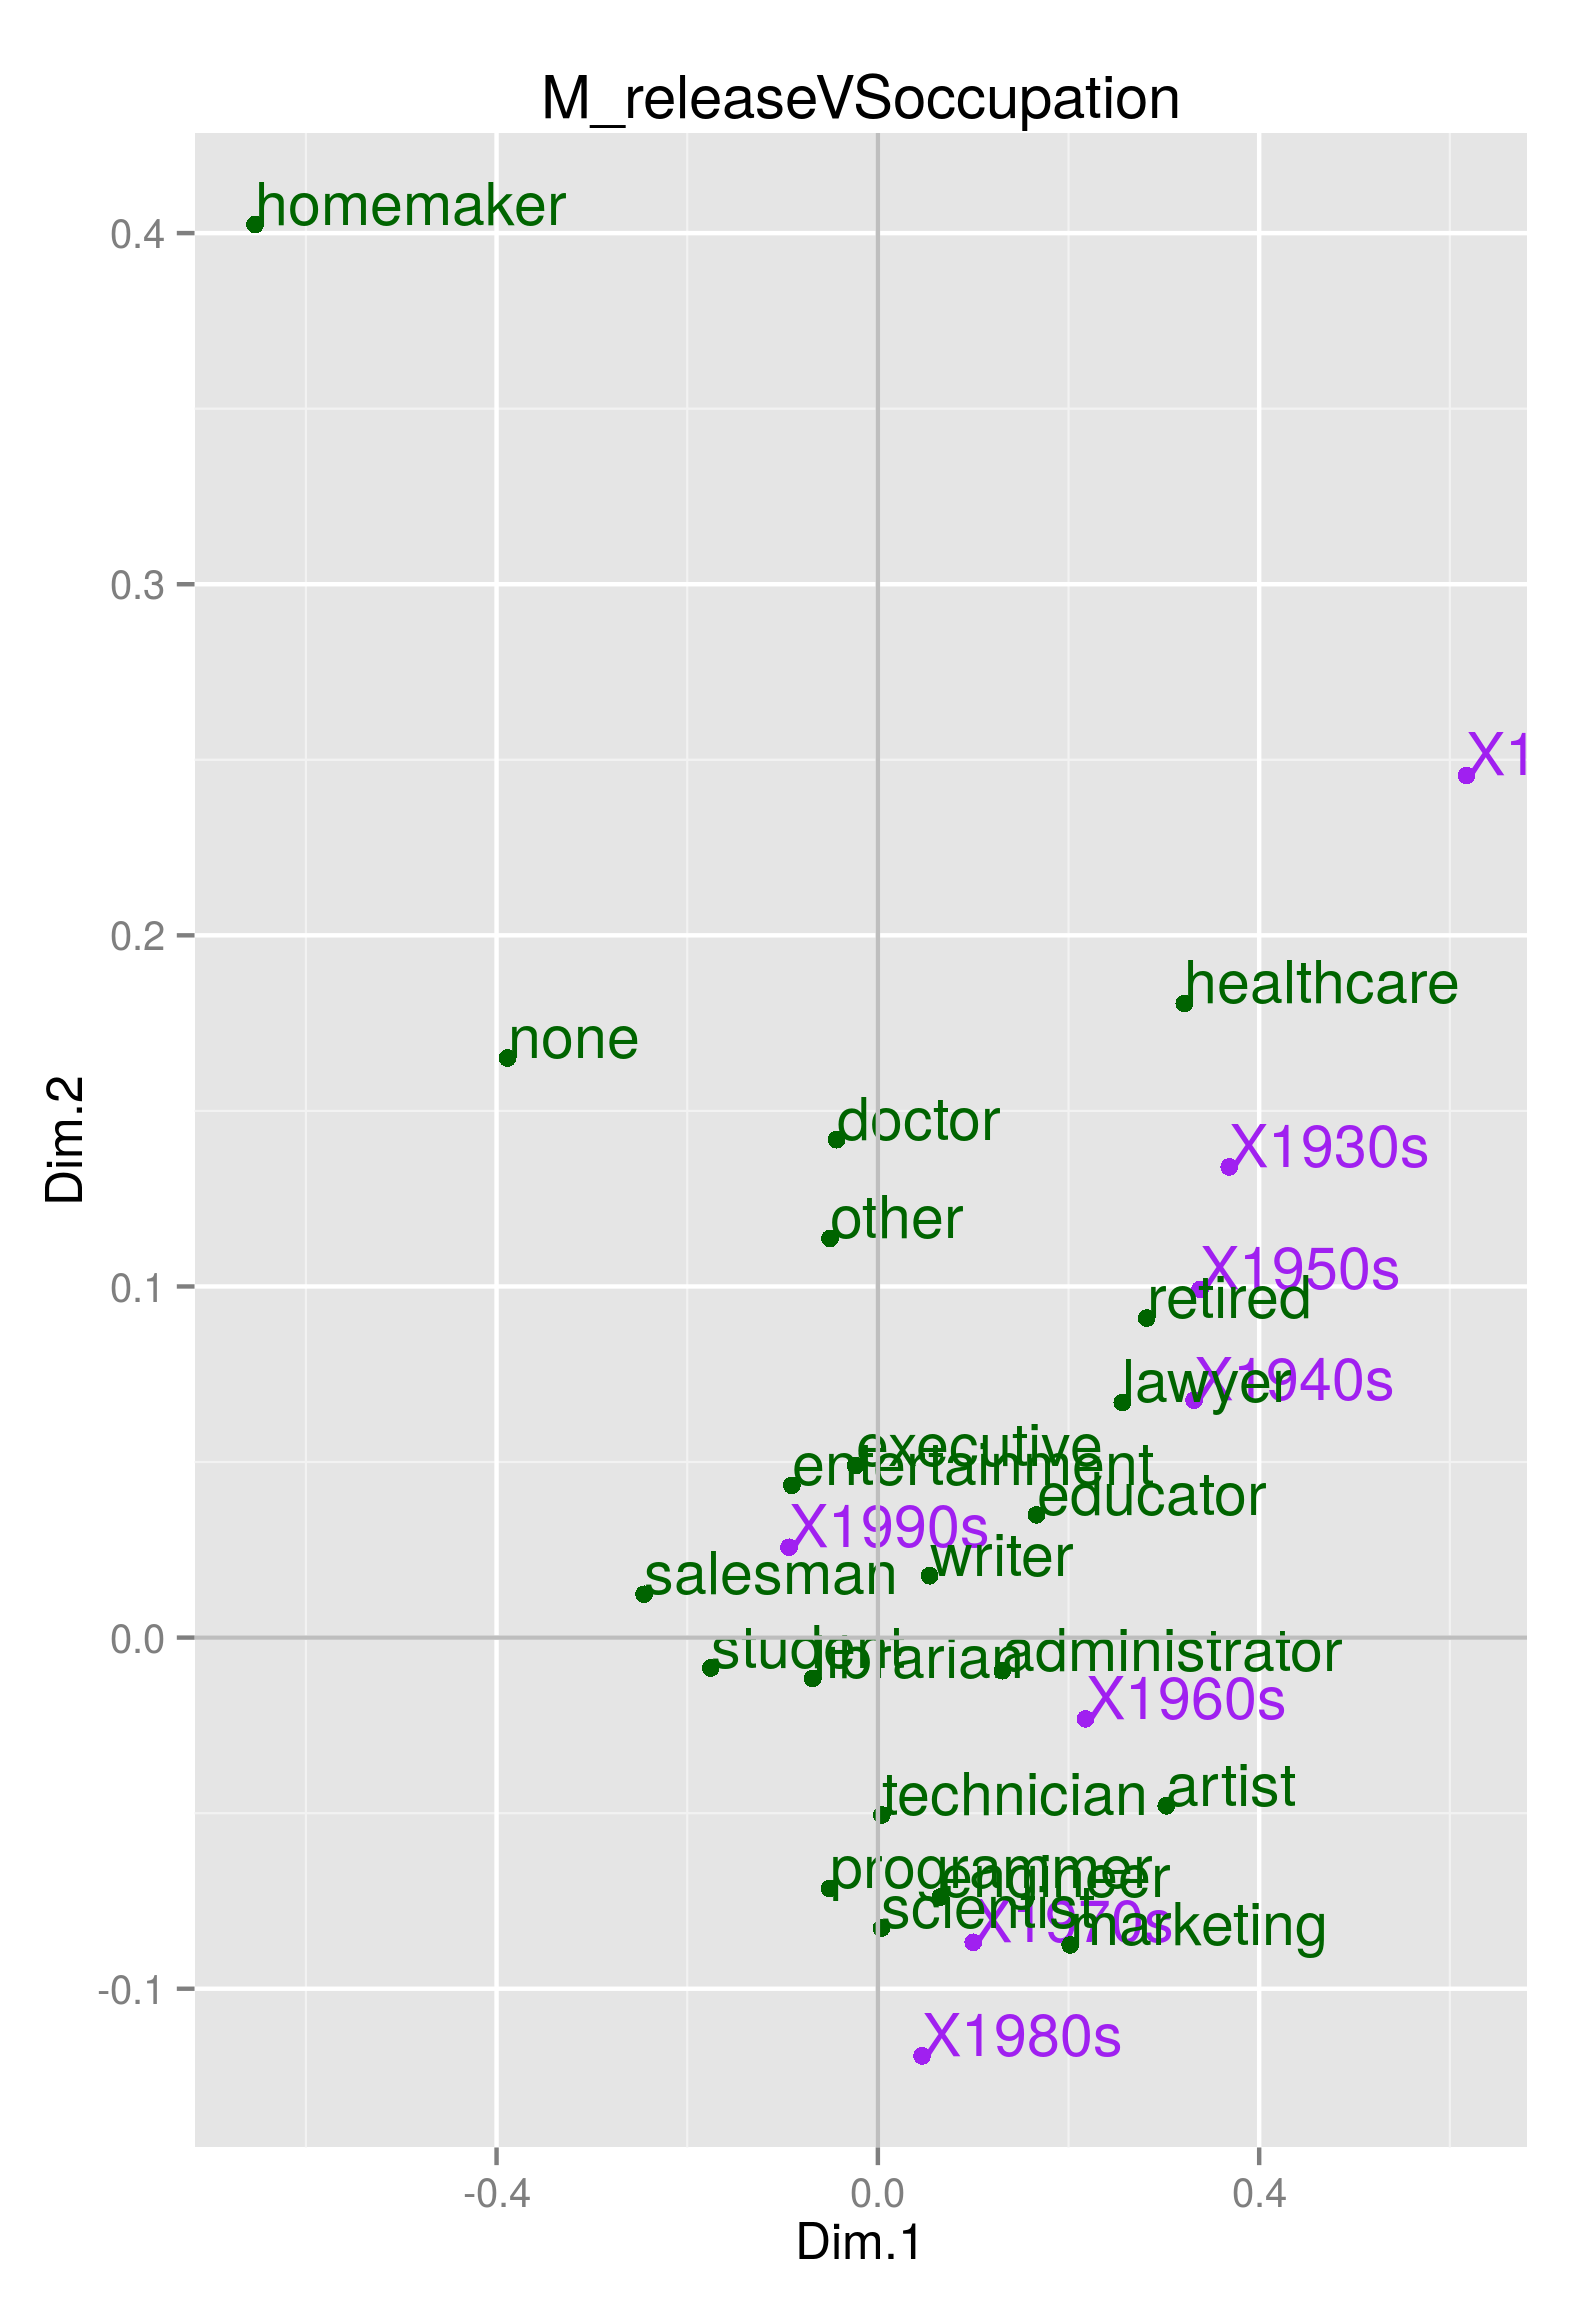
\includegraphics[scale=0.65]{./images/M_releaseVSoccupation}
\caption{Décennie de sortie des films par rapport à l'occupation professionnelle des utilisateurs}
\end{figure}

\pagebreak
\section{Décennie de sortie des films | Région d'habitation des utilisateurs}
\subsection{Femmes}
\begin{figure}[htd]
\centering
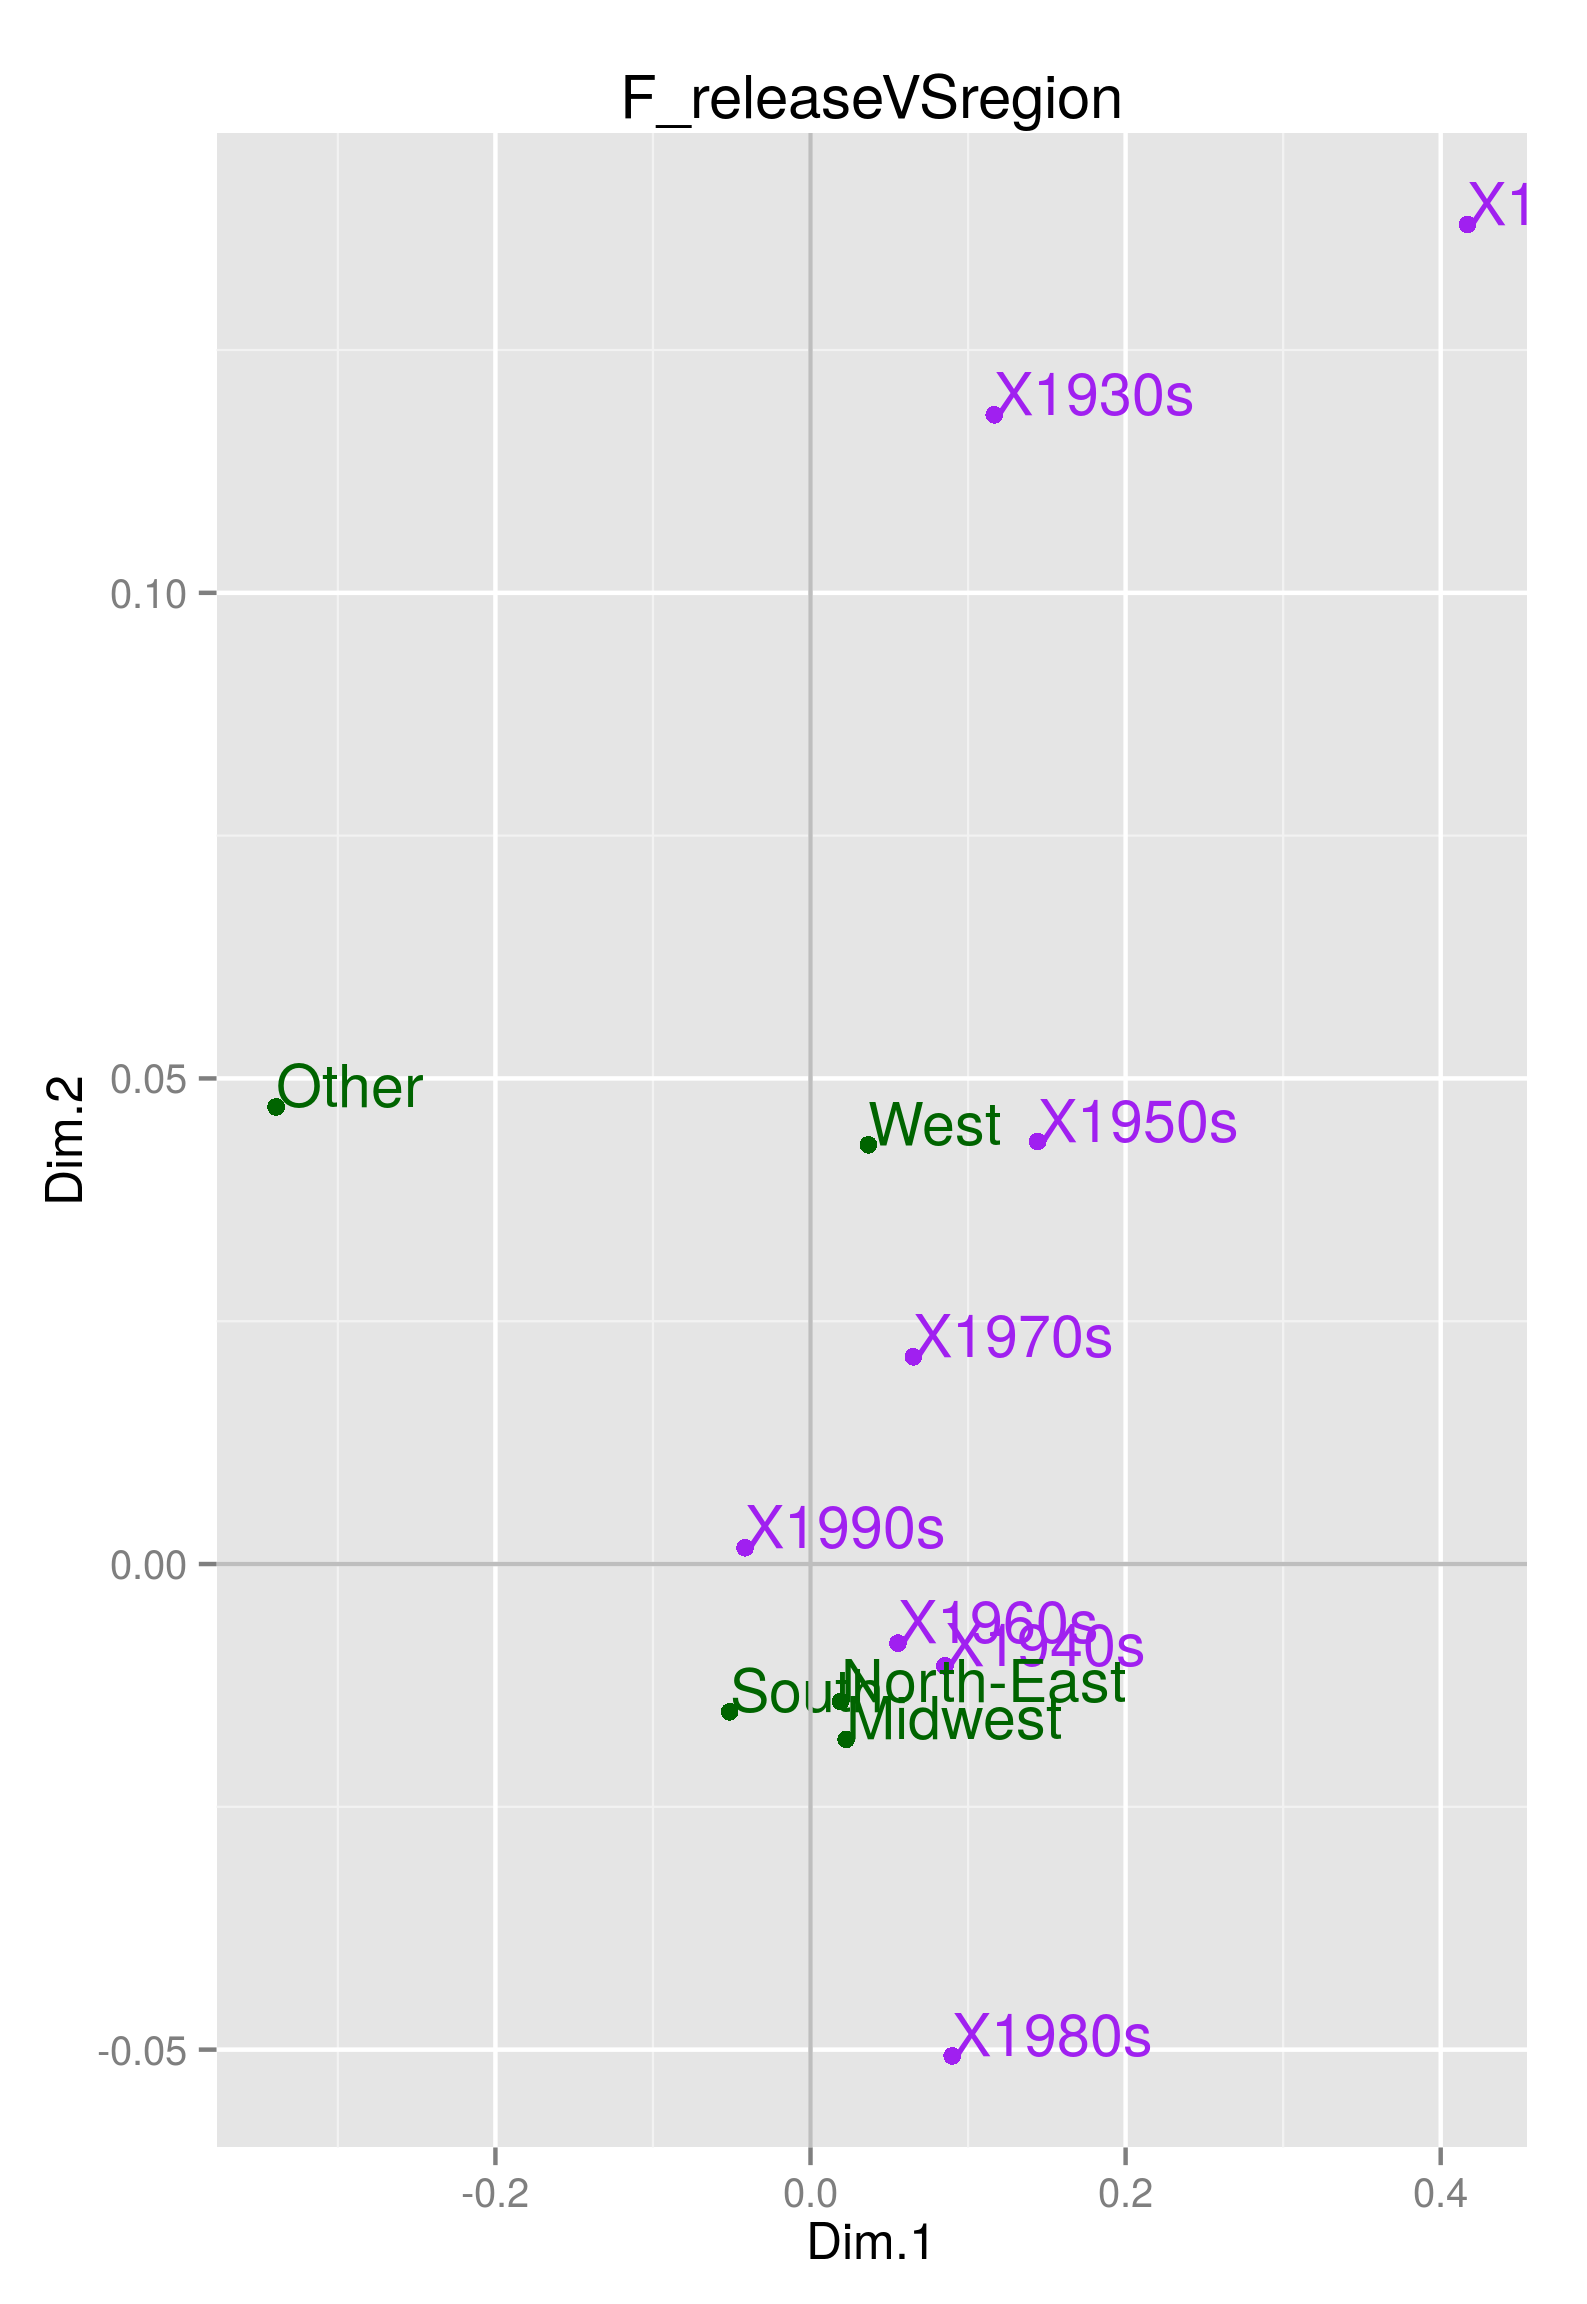
\includegraphics[scale=0.65]{./images/F_releaseVSregion}
\caption{Décennie de sortie des films par rapport à la région d'habitation des utilisatrices}
\end{figure}

\pagebreak
\subsection{Hommes}
\begin{figure}[htd]
\centering
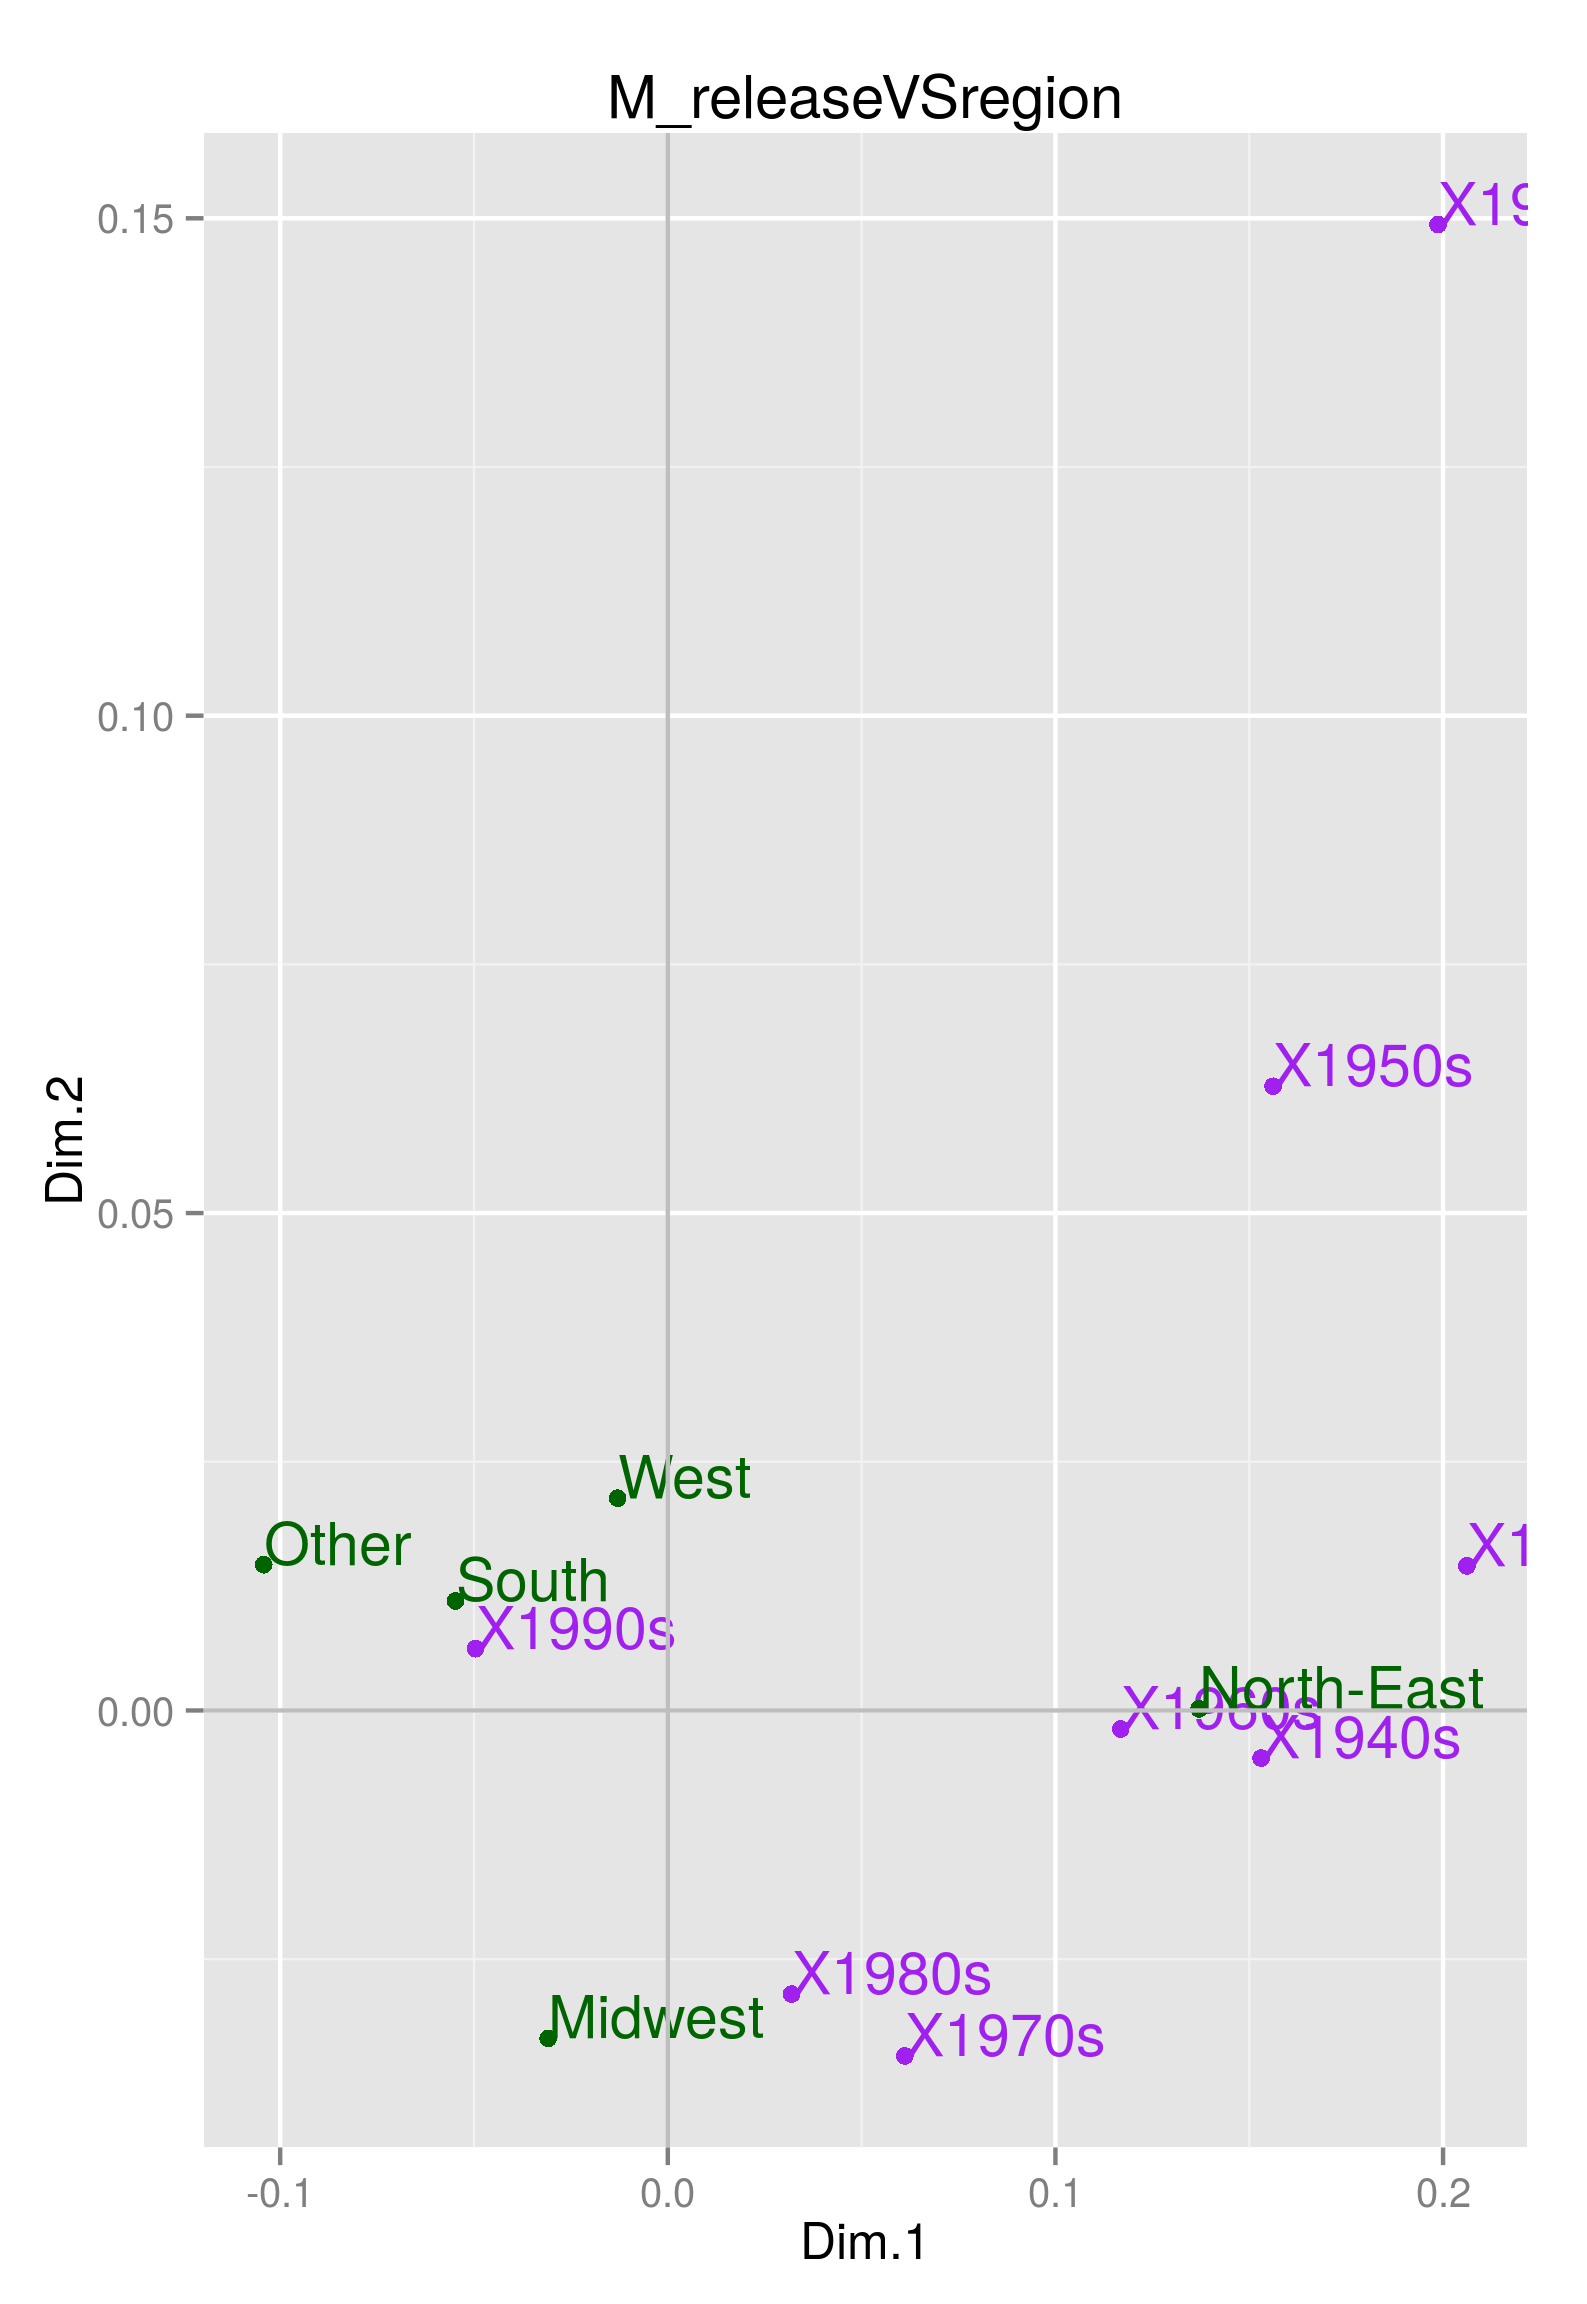
\includegraphics[scale=0.65]{./images/M_releaseVSregion}
\caption{Décennie de sortie des films par rapport à la région d'habitation des utilisateurs}
\end{figure}


\end{document}
